\documentclass[11pt]{article}

% ------------------------------------------------------------------ preamble
\usepackage[margin=1.0in]{geometry}
\usepackage{mathpazo}
\usepackage[T1]{fontenc}
\usepackage{microtype}
\usepackage{amsmath,amssymb}
\usepackage{graphicx}
\usepackage{booktabs}
\usepackage{caption}
\usepackage{tikz}
\usetikzlibrary{arrows.meta,positioning,shapes.geometric}
\usepackage[round]{natbib}
\usepackage{xcolor}
\usepackage[colorlinks=true,linkcolor=blue!50!black,citecolor=blue!50!black,urlcolor=blue!50!black]{hyperref}
\usepackage{enumitem}
\setlist{itemsep=2pt,topsep=4pt}

\captionsetup{font=small,labelfont=bf,width=0.92\textwidth}
\captionsetup[table]{position=above,skip=6pt}
\graphicspath{{figures/v2/}{figures/notebook/}}
\usepackage{placeins}
\usepackage{float}
\usepackage{fancyhdr}
\pagestyle{fancy}
\fancyhead[L]{\small\itshape Count Each Idea Once}
\fancyhead[R]{\small\itshape\nouppercase{\rightmark}}
\renewcommand{\sectionmark}[1]{\markboth{Count Each Idea Once}{\thesection\ \ #1}}
\renewcommand{\subsectionmark}[1]{\markright{\thesubsection\ \ #1}}
\fancyfoot[C]{\thepage}
\renewcommand{\headrulewidth}{0.3pt}
\setlength{\headheight}{14pt}
\widowpenalty=9000
\clubpenalty=9000

% keep floats near their text instead of piling up at the end
\renewcommand{\topfraction}{0.88}
\renewcommand{\bottomfraction}{0.7}
\renewcommand{\textfraction}{0.08}
\renewcommand{\floatpagefraction}{0.72}
\setcounter{topnumber}{3}
\setcounter{bottomnumber}{2}
\setcounter{totalnumber}{5}
\setlength{\textfloatsep}{11pt plus 2pt minus 3pt}
\setlength{\intextsep}{10pt plus 2pt minus 2pt}
\setlength{\abovecaptionskip}{6pt}
\captionsetup{width=0.95\textwidth}

\newcommand{\ic}{\mathrm{IC}}
\newcommand{\cone}{class~1}

\title{\textbf{Count Each Idea Once:\\ Building Robust Composites from\\ Correlated Alpha Signals}\\[1.2ex]
\large Berkeley MFE Industry Project, sponsored by Ultramarin}
\author{Hashim Almodamagha\\ \small Master of Financial Engineering, UC Berkeley Haas School of Business}
\date{July 2026}

\begin{document}

\maketitle

\begin{abstract}
\noindent
A quantitative research team rarely holds one definition of a factor. It holds a cluster of
correlated variants of the same idea, and those variants must somehow become one signal.
This report asks how such a cluster should be combined into a single composite, and whether
anything beats the benchmark of ranking each variant and averaging. On four anonymized
feature classes provided by Ultramarin (roughly 1{,}500--3{,}100 in-sample trading days
each, $\sim$390--480 names per day), I evaluate composition methods ranging from equal
weighting through supervised regressions, partial least squares, gradient-boosted trees,
redundancy-aware clustering, and a random-effects estimator borrowed from clinical
meta-analysis, under one fixed evaluation framework: daily rank information coefficients
with Newey--West significance, signal decay, factor turnover, and purged
cross-validation, followed by a final frozen test on a blind hold-out of roughly
2{,}180 unseen trading days per class. The resulting findings led to a robust
methodology supported by evidence. \emph{Count each idea once}: cluster near-duplicate variants into
blocks, average within each block, weight the blocks equally, add learned per-feature
transforms only where in-sample evidence clearly supports them, and freeze every parameter.
No method in the study, including this one, delivers more raw predictive accuracy than the
benchmark. What the selected composite improves is everything around the accuracy: it
matches the benchmark on every hold-out class while carrying the smallest worst-case loss
when the feature set is perturbed, and where the two differ it decays more slowly and trades
at 35--40\% lower turnover. In short, the methodology keeps only what the evidence supports, and documents why
every rejected alternative was left out.
\end{abstract}

\clearpage

% =====================================================================
\section{Introduction}
\label{sec:intro}

Feature definitions in finance are arbitrary in a specific, well-known way. The literature
settles on one definition of momentum, say twelve-month return skipping the most recent month,
but a live research process accumulates dozens: different lookbacks, different normalizations,
risk-adjusted and residualized flavors, each a noisy measurement of the same latent signal.
This report investigates how a large set of highly correlated features, all manifestations of
one signal theme, can be combined into a single robust composite, and whether any weighting
scheme can beat the simplest one.

That simplest scheme is the benchmark throughout this report: rank each variant
cross-sectionally, then average the ranks with equal weights. Writing $r_{j,t}$ for
variant $j$'s cross-sectional rank on day $t$ and $s_j$ for the sign of its
training-window IC, the benchmark composite on day $t$ is
\begin{equation}
F_t \;=\; \frac{1}{N}\sum_{j=1}^{N} s_j\, r_{j,t},
\label{eq:benchmark}
\end{equation}
where the sign flips any variant whose training relationship with the target is negative
(on percentile ranks a reflected variant differs from $-r_{j,t}$ only by a constant,
which no ranking sees). We refer to it as the \emph{benchmark} or the rank-and-average
composite. It is harder to beat than it looks, but
it has one structural flaw: it weights definitions, not ideas. For example, if eight of ten
variants are re-implementations of ``cumulative return,'' the average is really that one
idea, eight times over, with the other two ideas diluted to noise. The objective is
therefore a systematic, statistically sound way to weight variants by uniqueness and
information content rather than by how many near-duplicates happen to land in the cluster.

The textbook dimensionality-reduction answer, PCA, is unfortunately not the answer here.
PCA extracts the linear combination with maximum variance, while our objective is
maximum correlation with residualized forward returns, a target the PCA objective never
sees. On redundant clusters the two
disagree in exactly the wrong direction: the near-duplicates share most of the common
variance, so the first principal component concentrates on the most-repeated definition,
which reproduces the benchmark's flaw in a more roundabout form. The cost is measurable. On the
one class in our data with several distinct sub-themes, a frozen first-principal-component
composite keeps about a third of the benchmark's out-of-sample IC.

To answer the question systematically, I built a single fixed evaluation framework (daily
rank IC, Newey--West $t$-statistics, signal decay, factor turnover, purged $k$-fold
cross-validation) and pushed a sequence of composition methods of increasing complexity
through it: equal-weight and IC-weighted averages, GLS-style ``uniqueness'' regressions,
penalized regressions, partial least squares, gradient-boosted trees, cluster-then-weight
composites, and a tuning-free random-effects weighting borrowed from clinical meta-analysis.
Everything that survived in-sample scrutiny was then frozen and scored once on a blind
hold-out: roughly 2{,}180 trading days per class that arrived after all in-sample decisions
were locked. Two statistical checks close the study: a family-wise multiplicity correction
across all 56 method-versus-benchmark comparisons the project ever ran, and
estimator-robustness checks on the one data-driven decision the final method retains.

From the outset, the project favored transparent reporting over good-looking results, and
that mandate shaped it more than any single method did. Three findings define the story.

\begin{enumerate}
\item Each cluster is worth what it is worth, and no weighting scheme extracts more.
      Every class has a hard IC ceiling (0.031 for the strongest, 0.015 for the weakest) that
      equal weighting essentially attains and that trees, PLS, GLS, and tuned penalties cannot
      move. After multiplicity correction, no method in the study beats the benchmark on
      raw IC (Section~\ref{sec:referee}).
\item Deduplication is the one idea that survives every test. Clustering the
      variants, collapsing each redundancy block to its sign-aligned average, and
      weighting blocks equally matches the benchmark everywhere while never being the
      casualty: it has the shallowest worst case across 80 random feature-subset
      perturbations, no blow-up on any hold-out class, and the study's only nominally
      significant win against the benchmark (on the multi-factor class, where the
      benchmark's duplication bias actually binds).
\item The selected composite's edge is signal quality, not the level of its IC.
      Every class has its own ceiling, and the selected composite sits at or within noise
      of all four of them, which no single rival method manages: trees collapse off
      class~1, regression fits invert on class~3, and PCA collapses on class~4. Where a
      class has learnable shape structure the composite adds it, and it then holds its IC
      at longer holding horizons at materially lower factor turnover, so it trades more
      cheaply than the benchmark wherever the two differ at all.
\end{enumerate}

% =====================================================================
\FloatBarrier
\section{Related work}
\label{sec:related}

Combining correlated noisy predictors of one quantity is the oldest problem in the
forecasting literature \citep{bates1969,clemen1989,timmermann2006}. Its most robust
empirical finding, the ``forecast combination puzzle,'' is that estimated ``optimal''
weights routinely lose to equal weights out of sample, because the weights themselves are
estimated with error comparable to the differences they chase \citep{stock2004,smith2009}.
The portfolio-choice analogue is \citet{demiguel2009}: no estimated allocation consistently
beats $1/N$. Our study effectively replays this literature inside a single alpha signal,
and reaches the same resolution the literature does: shrink toward equal weights, and
deviate only on strong evidence. What we add is the deduplication observation. On redundant
clusters the right unit for ``equal'' is the idea (the redundancy block), not the raw
variant, a distinction the classical combination literature does not need because its
forecasters are not near-duplicates.

The mechanism behind the puzzle has a name and a remedy. It is the Stein phenomenon
\citep{james1961,efron1977}: when many means are estimated jointly, shrinking toward a
common value dominates the raw estimates, and Ledoit--Wolf covariance shrinkage
\citep{ledoit2004} applies the same logic to covariance matrices. Both appear in our results
in recognizable form. The ``uniqueness'' regression of Section~\ref{sec:methods-linear}
only works when its ridge penalty is large, that is, when it stops trusting the estimated
covariance, and the random-effects estimator of Section~\ref{sec:methods-dl} is exactly a
James--Stein shrinkage of per-block ICs with a data-estimated intensity.

The cleanest off-the-shelf implementation of that shrinkage idea comes from an unexpected
field. Pooling $k$ correlated, noisy effect estimates is the core problem of research
synthesis in medicine \citep{cochran1954,borenstein2010}, and the random-effects model of
\citet{dersimonian1986} estimates the between-study heterogeneity $\tau^2$ in closed form,
interpolating between equal weighting ($\tau^2=0$) and precision weighting ($\tau^2$
large). We import it as a tuning-free adaptive weighting across redundancy blocks, with
alternative $\tau^2$ estimators \citep{paule1982,harville1977,veroniki2016} and the
Hartung--Knapp small-$k$ correction \citep{hartung2001} as robustness checks in
Section~\ref{sec:referee}. To our knowledge the explicit mapping (feature variant as study,
train-window IC as effect estimate, Newey--West standard error as within-study error,
duplicated definitions as duplicate publications) is not standard in the signal-combination
literature, and Section~\ref{sec:methods-dl} spells it out.

Whatever the weighting scheme, the evaluation has to be trustworthy, and here we follow the
standard institutional playbook: information coefficients and the breadth arithmetic of
\citet{grinold2000}; HAC standard errors \citep{newey1987}, because overlapping 21-day
targets induce strong serial correlation in daily ICs; and purged $k$-fold cross-validation
with embargo \citep{lopezdeprado2018}, because random splits leak overlapping labels. A
research process that runs many backtests will find ``significant'' ones by construction,
the multiplicity problem of \citet{harvey2016}. We implement their prescription literally
in Section~\ref{sec:referee}, with Holm \citep{holm1979}, Benjamini--Hochberg
\citep{benjamini1995}, and the dependence-aware Westfall--Young max-$T$ bootstrap
\citep{westfall1993} over every comparison the project ever ran.

Finally, the nonlinear probes use gradient boosting \citep{friedman2001,chen2016,ke2017}.
The finding that a depth-1 (stump) ensemble, exactly a generalized additive model
\citep{hastie1986}, reproduces everything the deeper trees deliver places our results in a
familiar tradition: on tabular financial data the win, when there is one, is per-feature
nonlinearity, not interactions. The two-compartment decay decomposition mentioned in
Section~\ref{sec:insample-trees} borrows its functional form from pharmacokinetics
\citep{gibaldi1982}.

% =====================================================================
\FloatBarrier
\section{Data and exploratory analysis}
\label{sec:data}

\subsection{The panels}
\label{sec:data-panels}

Ultramarin provided four anonymized \emph{feature classes}, referred to as class~1 through
class~4 throughout this report. Each class is one cluster of correlated feature variants
$f_1,\dots,f_N$, delivered as within-day cross-sectional ranks on a panel of anonymized
equity identifiers. Each $f_j$ is, at least in principle, a representation of the same
latent feature. Alongside the variants comes a single target: residualized forward returns.
Dates are integer-indexed trading days, and identifiers are anonymized but consistent
within a class. Table~\ref{tab:data} summarizes the panels after preprocessing to complete
cases, that is, dropping rows with a missing target or any missing variant. This removes
under 0.4\% of rows for classes 1 and 4 and about 12\% for classes 2 and 3 in sample, and
under 1\% everywhere on the hold-out.

\begin{table}[H]
\centering
\small
\caption{The four feature classes. ``PC1 var.\ share'' is the fraction of within-class
feature variance explained by the first principal component of the pooled panel correlation
matrix of the variants (all days stacked, one correlation matrix per class, not a
day-by-day PCA): a measure of how close the cluster is to one factor. The blind hold-out
(Section~\ref{sec:holdout}) is the immediately following period for every class and was
delivered only after all in-sample analysis was frozen.}
\label{tab:data}
\begin{tabular}{lrrrrrrr}
\toprule
 & variants & \multicolumn{2}{c}{in-sample} & \multicolumn{2}{c}{hold-out} & names/day & PC1 var.\ share \\
 & & days & rows & days & rows & & \\
\midrule
class 1 & 16 & 3{,}130 & 1.51M & 2{,}195 & 0.93M & $\sim$481 & 0.48 \\
class 2 & 10 & 1{,}565 & 0.61M & 2{,}195 & 0.93M & $\sim$390 & 0.51 \\
class 3 &  6 & 1{,}565 & 0.61M & 2{,}195 & 0.93M & $\sim$390 & 0.53 \\
class 4 & 20 & 3{,}130 & 1.51M & 2{,}195 & 0.93M & $\sim$481 & 0.30 \\
\bottomrule
\end{tabular}
\end{table}

\subsection{The target}
\label{sec:data-horizon}

The target we model is a residualized cumulative forward return over approximately 21
trading days (one month), sampled every day. Because consecutive days' targets share 20 of
their 21 forward days, the target's autocorrelation decays linearly to zero at lag 21
(Figure~\ref{fig:target}). Its cross-sectional dispersion, the standard deviation of the
target across names on a given day, is about 6.6\% and annualizes to a sensible
$\sim$23\% only at the monthly horizon, consistent with a monthly return sampled daily.
This overlap is the one property of the target that matters for everything downstream: it
fixes the 21-day purge-and-embargo window in cross-validation and the 25-lag width of every
Newey--West standard error in the study.

\begin{figure}[!tbp]
\centering
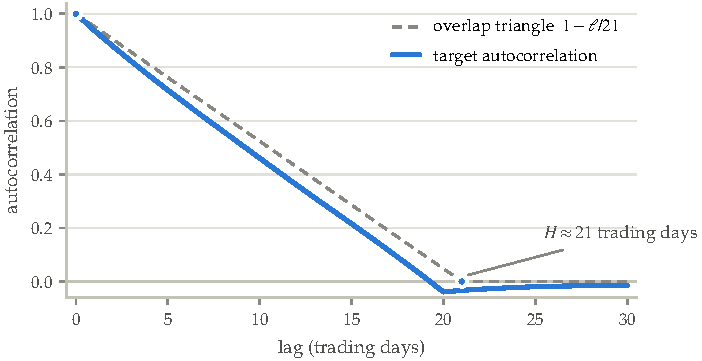
\includegraphics[width=0.58\textwidth]{fig_target.pdf}
\caption{The returns being modeled. The target's autocorrelation traces the overlap triangle
of a $\sim$21-day cumulative forward return sampled daily; this one property sets the purge
window and the HAC lag count for the entire study.}
\label{fig:target}
\end{figure}

\subsection{Redundancy and orientation}
\label{sec:data-redundancy}

Before any averaging is meaningful, all variants in a cluster must point the same way
relative to the target. That requirement cannot be met by feature-to-feature correlations
alone, which are themselves noisy and say nothing about which direction predicts. A minimal
level of supervision is therefore unavoidable: at least one sign per cluster must come from
the target, and in the composites below every variant is ultimately flipped by the sign of
its training-window IC. What unsupervised structure can still tell us is how the variants
relate to each other, and that is what this section examines.

Figure~\ref{fig:threeview} shows each class's correlation matrix three ways: raw, grouped by
sign convention, and grouped by redundancy after \emph{sign alignment}. Alignment reflects a
variant ($x \mapsto 1-x$ on percentile ranks) if and only if it loads negatively on the
cluster's first principal component, a convention fix that changes no correlation magnitude.
The three views separate two things that are easy to conflate.

\begin{itemize}
\item Orientation. Class~1 looks like a mixed positive/negative grid, but flipping
      just 2 of its 16 variants collapses it into a single coherent positive block (mean
      off-diagonal correlation 0.21 $\to$ 0.44, negative-pair fraction 0.23 $\to$ 0). One
      theme, inconsistent sign conventions. Classes 2 and 3 arrive already coherent.
\item Real multi-factor structure. Class~4 is an exception to the others: five
      variants get flagged, but flipping them does not clean the matrix (mean
      off-diagonal actually falls, 0.23 $\to$ 0.15). Its negative correlations are real
      disagreement between sub-themes, not reversed duplicates. This is the cluster where
      uniqueness-aware weighting should finally earn its keep, and the one where it
      eventually (nominally) does. It is also exactly the case the prerequisite above
      predicts: when a cluster is not one theme, a PC1-based sign convention cannot
      substitute for target-based signs, and it is the training-IC sign bits that
      resolve class~4.
\end{itemize}

Within-class redundancy is otherwise exactly as the project premise describes: solid blocks
of 0.7--0.95 correlation, many variants being near-duplicate re-implementations, and this
duplication is precisely what the benchmark overweights. Two further exploratory facts
constrain what follows. First, within a class the variants' $|\ic|$ values are broadly
similar. No definition dominates, so sophisticated weighting has little cross-sectional
signal to exploit and must still pay its estimation noise. Second, class~1 illustrates why
the target's sign bit is irreducible: after alignment its coherent orientation is
\emph{anti-predictive}, with all 16 variants carrying negative IC. A purely unsupervised
composite of this cluster is not just weaker, it points the wrong way.

\begin{figure}[!tbp]
\centering
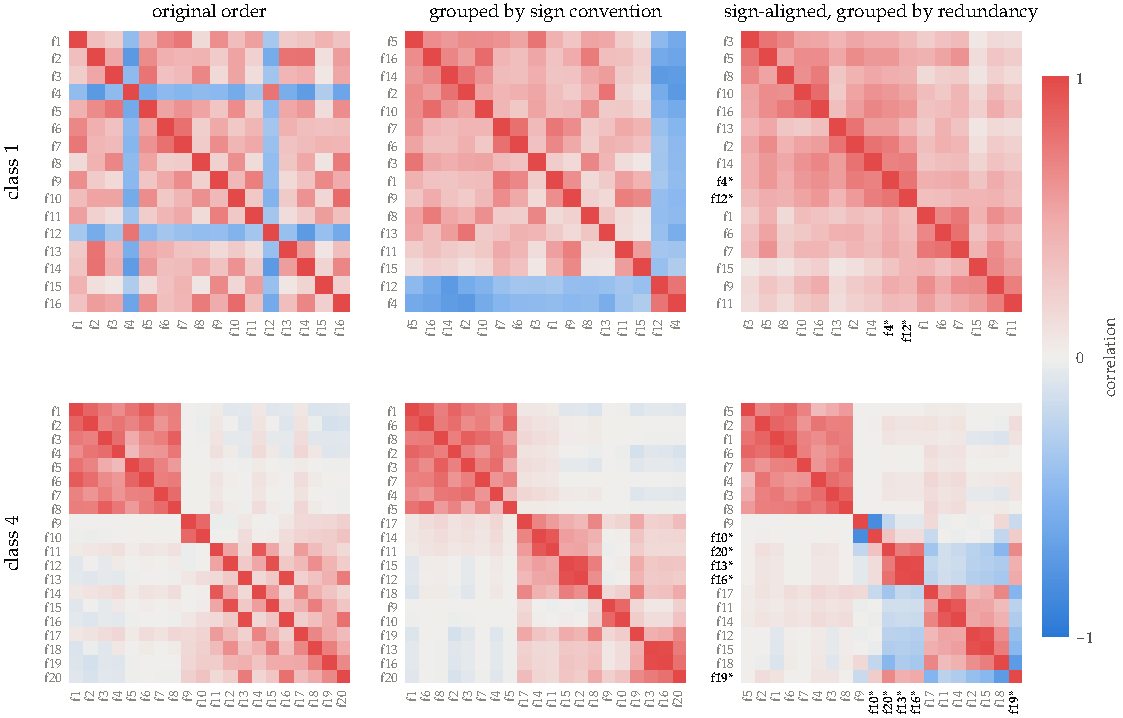
\includegraphics[width=0.86\textwidth]{fig_threeview.pdf}
\caption{The two classes that carry the orientation story: correlation matrices raw (left),
grouped by sign convention (middle), and sign-aligned then grouped by redundancy (right;
$*$ marks reflected variants). Class~1 (top) collapses to one coherent block after flipping
two variants; class~4 (bottom) retains real sub-block structure that no per-feature sign
fix can reconcile. Classes 2--3 arrive already coherent.}
\label{fig:threeview}
\end{figure}

% =====================================================================
\FloatBarrier
\section{Evaluation framework}
\label{sec:framework}

Every method in this study is scored by a fixed set of metrics, defined before any
comparison was run. On day $t$, let $F_t$ be the cross-section of composite scores and
$R_t$ the matching realized targets. The day's \emph{information coefficient} is the
Spearman rank correlation
$\ic_t = \mathrm{corr}\bigl(\mathrm{rank}(F_t), \mathrm{rank}(R_t)\bigr)$. The focus on
ranks is a scope decision, not a claim of universality: this study evaluates signals as
orderings, which is robust to fat-tailed returns, while portfolio constructions that use
the distance between predictions lie outside its scope. Daily equity ICs are small
(0.02--0.05 is a strong signal), and all inference runs on the time series $\{\ic_t\}$
through the following metrics:

\begin{center}
\small
\begin{tabular}{lll}
\toprule
metric & definition & reads as \\
\midrule
mean IC & $\overline{\ic_t}$ & average daily predictive strength \\
IC-IR & $\overline{\ic}/\mathrm{std}(\ic_t)$ & risk-adjusted consistency \\
Newey--West $t$ & mean IC over its HAC (25-lag) s.e. & significance under serial correlation \\
hit rate & fraction of days with $\ic_t>0$ & sign robustness check \\
signal decay & $\mathbb{E}[\ic(F_{t-l},R_t)]$ vs.\ lag $l$ & shelf life of the signal \\
factor turnover & $\mathbb{E}[\mathrm{corr}(F_{t-l},F_t)]$ & trading cost proxy \\
\bottomrule
\end{tabular}
\end{center}

To ensure the integrity and soundness of our results, three procedures guard every
comparison in the study.

\paragraph{HAC significance.} Because the target is a 21-day overlapping return, daily ICs
are strongly serially correlated and uncorrected standard errors overstate significance
several-fold. Every $t$-statistic in this report is Newey--West with 25 lags, wide enough to
absorb the overlap established in Section~\ref{sec:data-horizon}.

\paragraph{Purged cross-validation.} All in-sample method comparisons use 5-fold
cross-validation on contiguous chronological day blocks, never splitting a day's
cross-section, with a 21-day purge and embargo around each test block so no training label's
forward window reaches into test days. Random row splits on overlapping labels are textbook
leakage, and blocked splits with purging avoid it. Every tuned hyperparameter
($\lambda$, $\rho$, PLS-$k$, tree count) is chosen on an inner chronological
validation slice of the training window, by validation rank IC, never on the test fold.

\paragraph{Paired tests, out of fold.} A method never gets credit for its in-sample fit.
Claims of the form ``$A$ beats $B$'' are adjudicated by a paired Newey--West test on the
out-of-fold daily IC difference series $\ic^A_t - \ic^B_t$: same days, same folds.
This discipline pays for itself early. XGBoost's apparent in-sample IC edge (0.047 vs.\
0.031) evaporates the moment it is scored out of fold
(Section~\ref{sec:insample-ceiling}).

Finally, the entire in-sample study was conducted before the blind hold-out was
delivered; Section~\ref{sec:holdout} describes the freeze protocol under which it was scored
exactly once.

% =====================================================================
\FloatBarrier
\section{Methods}
\label{sec:methods}

The candidate methods are organized from simplest to most complex, and each addition must
justify itself against the simpler alternatives under the framework of
Section~\ref{sec:framework}.

\subsection{Baselines and linear weightings}
\label{sec:methods-linear}

\begin{itemize}
\item \emph{Benchmark.} Flip each variant by the sign of its train IC, then
      equal-weight average the ranks. The rank-and-average composite of
      Section~\ref{sec:intro}.
\item \emph{PCA PC1.} The first principal component, oriented target-free to agree
      with the benchmark, which carries the cluster's one train-IC sign bit
      (Section~\ref{sec:data-redundancy}). The unsupervised straw man, retained precisely
      so its failure is measured, not assumed.
\item \emph{IC weighting.} Weights proportional to each variant's train-window IC:
      weight by signal, ignore redundancy. For standardized features this coincides with
      the first partial-least-squares direction. In our testing it is applied both to
      raw features and to the cluster blocks of Section~\ref{sec:methods-cluster}.
\item \emph{Uniqueness regression.} Weights proportional to
      $(\Sigma+\lambda I)^{-1}\hat{\imath}$, where $\Sigma$ is the correlation matrix of
      the variants, $\hat{\imath}$ is the vector of their train-window ICs, $I$ is the
      identity matrix, and $\lambda \ge 0$ is a ridge penalty. This is a regularized
      GLS direction that down-weights redundant variants, the literal implementation of
      ``weight by uniqueness and information content.'' Both a tuned-$\lambda$ and a
      fixed-$\lambda$ version are tested.
\item \emph{OLS, ridge, lasso.} Textbook cross-sectional regressions (predict, then
      rank), with leak-free inner-validation tuning.
\item \emph{PLS.} Partial least squares with the number of components $k$ tuned on
      inner validation, asking how many supervised directions the cluster holds.
\item \emph{Boosted trees.} XGBoost and LightGBM in a deliberately low-capacity
      configuration (depth 3, slow learning rate, only the tree count tuned), asking
      whether there is structure a linear combination cannot see.
\end{itemize}

\subsection{Cluster-then-weight composites}
\label{sec:methods-cluster}

The second family tackles duplication directly: cluster the variants by average-linkage
hierarchical clustering on $1-|\mathrm{corr}|$, merging variants whose absolute correlation
is at least a threshold $\rho$, collapse each resulting redundancy block to its
sign-aligned average, then weight the \emph{blocks}. Three block weightings are tested:
equal weights, weighting by block train ICs, and a GLS solve across blocks. The clustering step is the hard form of an
equal-weight prior. Rather than penalizing weight dispersion continuously (a tuned
diversification penalty, also tested, also failed), it injects the structure we actually
believe: the same idea implemented twice should count once. The merge threshold is fixed at
$\rho=0.7$, at which two merged variants share roughly half their variance. Sections
\ref{sec:insample-stress} and \ref{sec:holdout} show that leak-free tuning of $\rho$, offered
repeatedly, never beats the fixed value. Figure~\ref{fig:dendro} draws the four merge trees
with this cut in place: across the classes, 52 variants collapse to 23 ideas.

\begin{figure}[H]
\centering
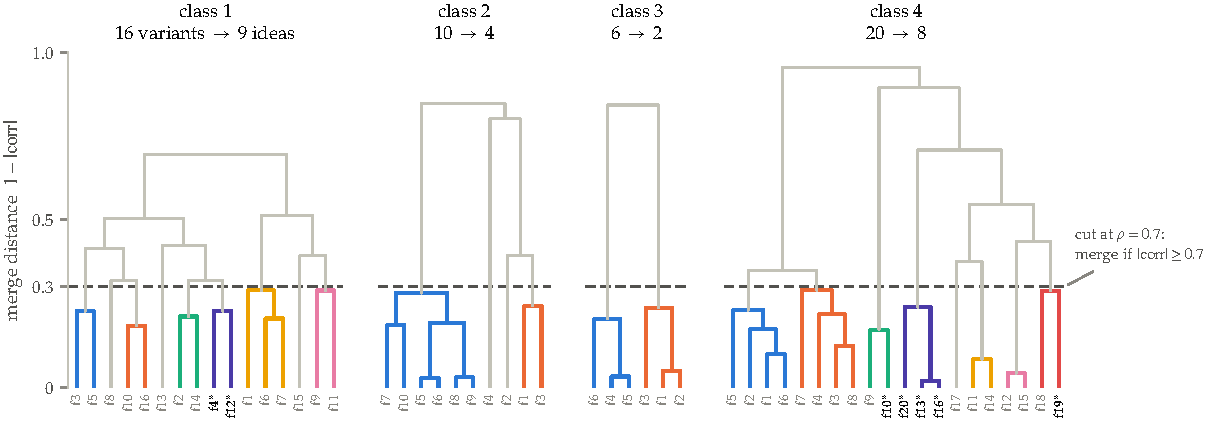
\includegraphics[width=0.98\textwidth]{fig_dendro.pdf}
\caption{The recipe's merge trees. Average-linkage dendrograms on $1-|\mathrm{corr}|$ for
each class, computed on the sign-aligned in-sample panel; the dashed line is the fixed merge
threshold $\rho=0.7$. Colored subtrees are the resulting redundancy blocks (colors
distinguish blocks within a class); gray leaves reaching the cut alone are already-unique
ideas. Across the four classes, 52 variants collapse to 23 ideas. Asterisks mark
sign-reflected variants (Section~\ref{sec:data-redundancy}); the tree itself uses absolute
correlation and is orientation-invariant.}
\label{fig:dendro}
\end{figure}

\subsection{A tuning-free adaptive weight, borrowed from medicine}
\label{sec:methods-dl}

Two weighting regimes emerge from the in-sample results below: equal block weights fit
one-factor clusters, and IC-tilted weights look better where blocks truly differ.
Choosing between them by validation search mostly measures luck. What we want instead is
a weight that adapts by estimation, and that is a solved problem in another field.

Combining $k$ noisy estimates of a common quantity is what meta-analysis does in clinical
medicine: each study $i$ reports an effect estimate $\hat\theta_i$ with standard error
$se_i$, and the analyst must pool them. The mapping onto our problem is exact:

\begin{center}
\small
\begin{tabular}{ll}
\toprule
meta-analysis & feature composition \\
\midrule
study $i$ & redundancy block $i$ (or variant $i$) \\
effect estimate $\hat\theta_i$ & block's train-window mean daily rank IC \\
within-study s.e.\ $se_i$ & Newey--West (25-lag) s.e.\ of that mean \\
duplicate publications of one trial & re-implemented definitions of one idea \\
fixed-effect pooling ($w_i \propto 1/se_i^2$) & $\approx$ IC-weighting \\
forcing equal $w_i$ & the benchmark \\
\bottomrule
\end{tabular}
\end{center}

The import is the \emph{random-effects} model of \citet{dersimonian1986} (henceforth DL). It
assumes the true per-block effects scatter with variance $\tau^2$ (the ``heterogeneity'')
around a grand mean, and estimates $\tau^2$ in closed form from the observed dispersion:
\begin{equation}
Q=\sum_{i=1}^{k} w_i(\hat\theta_i-\bar\theta)^2,\qquad
\hat\tau^2=\max\!\Bigl(0,\;
\frac{Q-(k-1)}{\sum_i w_i-\sum_i w_i^2/\sum_i w_i}\Bigr),\qquad w_i=1/se_i^2 .
\label{eq:dl}
\end{equation}
Here $k$ is the number of blocks, $\hat\theta_i$ is block $i$'s train-window mean daily
rank IC, $se_i$ is its Newey--West standard error, $w_i$ is the corresponding
precision weight, $\bar\theta=\sum_i w_i\hat\theta_i/\sum_i w_i$ is the
precision-weighted grand mean, and $Q$ measures how much the block ICs disperse around
that mean relative to their own noise. Each block IC is then shrunk toward the grand mean
and the blocks are weighted by the shrunk values:
\begin{equation}
\tilde\theta_i \;=\; \bar\theta + \lambda_i\,(\hat\theta_i-\bar\theta),
\qquad
\lambda_i=\frac{\hat\tau^2}{\hat\tau^2+se_i^2},
\qquad
\text{block weight} \;\propto\; \tilde\theta_i ,
\label{eq:dl-shrink}
\end{equation}
where $\lambda_i \in [0,1]$ is the reliability factor of the James--Stein /
empirical-Bayes form: it is 0 when the estimated heterogeneity is zero and approaches 1
when a block's IC is measured much more precisely than the blocks differ.

The estimator delivers the adaptivity we wanted with zero tuned hyperparameters, and for a
simple reason. The statistic $Q$ asks one question: is the spread of the block ICs larger
than their own standard errors would generate if every block carried identical
information? If not ($\hat\tau^2 = 0$), we cannot tell the blocks apart, every
$\lambda_i$ is 0, and equal weights fall out automatically. If yes ($\hat\tau^2 > 0$),
the differences are real signal, the shrinkage releases them, and the weights tilt toward
the higher-IC blocks. The estimator weights by measured information content precisely to
the degree the measurement itself is trustworthy. Econometrics knows the same phenomenon
as the forecast-combination puzzle, and medicine got there first with a closed form.

The resulting candidate, referred to below as the \emph{adaptive-weight} variant of the
dedup composite, runs this estimator across redundancy blocks: deduplicate first, then
pool, the correlated-studies discipline of the meta-analysis handbooks. A sibling variant
runs it on raw variants instead, deliberately re-admitting the duplicate-publication bias
so its cost can be measured.

\subsection{Learned feature shapes}
\label{sec:methods-shapes}

Every method so far consumes the variants as delivered: a stock's percentile rank enters
the composite untouched. That carries a silent assumption, namely that a gap in rank
means the same thing everywhere in the ranking, so that moving a stock from the 50th to
the 55th percentile is exactly as informative as moving it from the 93rd to the 98th.
Shape learning asks whether that assumption is true, by letting the data redraw the curve
each variant is read through and seeing whether it comes out straight. The instrument is
the simplest tree there is, a stump. A depth-1 stump is a one-variant, one-threshold rule (is this
variant's percentile above 0.83? if so, nudge the prediction up a step), and because
every stump touches a single variant, a boosted ensemble of stumps is exactly a
generalized additive model,
\begin{equation}
f(x) \;=\; c + \sum_{j=1}^{N} g_j(x_j),
\label{eq:gam}
\end{equation}
where $c$ is a constant and each $g_j$ is a one-dimensional response curve: all the
steps that reference variant $j$, stacked into one staircase, extractable from the fitted
ensemble in closed form as a lookup table. The tree probes (Section~\ref{sec:insample-trees}) locate XGBoost's one real
contribution in precisely these \emph{learned additive per-feature transforms}, and the
shaped composite keeps only the curves. Each variant is passed through its learned curve
as a preprocessing step, and the cluster composite of
Section~\ref{sec:methods-cluster} is then applied to the transformed variants unchanged:
\begin{equation}
\tilde{x}_j \;=\; g_j(x_j), \qquad
F^{\text{shaped}}_t \;=\; F^{\text{dedup}}_t\bigl(\tilde{x}_1,\dots,\tilde{x}_N\bigr).
\label{eq:shaped}
\end{equation}
Because the shapes represent 600 boosting rounds of extra capacity, they are adopted per
class only behind a mechanical \emph{evidence gate}, defined from in-sample quantities
only, with two stages and no tuned constants. Writing $t_{\mathrm{NW}}$ for the paired
Newey--West statistic of the shaped arm's out-of-fold daily IC against the unshaped
arm's, and $\mathrm{ret}_5$ and $\mathrm{turn}_5$ for the in-sample 5-day IC retention
and 5-day factor turnover, a class adopts shapes only if
\begin{equation}
\text{(A)}\;\; t_{\mathrm{NW}} > -2
\qquad\text{and}\qquad
\text{(B)}\;\; \mathrm{ret}_5^{\text{shaped}} > \mathrm{ret}_5^{\text{linear}}
\;\;\text{and}\;\;
\mathrm{turn}_5^{\text{shaped}} < \mathrm{turn}_5^{\text{linear}}.
\label{eq:gate}
\end{equation}
Condition (A) is a non-inferiority bar on accuracy under the purged CV, and condition
(B) demands a strict improvement on both tradeability measures at once. Condition (B)
encodes an asymmetry a plain accuracy comparison misses: shapes are only worth their
extra capacity where the linear composite actually churns.

% =====================================================================
\FloatBarrier
\section{In-sample results}
\label{sec:insample}

This section reports the in-sample study in the order it was actually run, because each
step's result determined the next. Section~\ref{sec:insample-ceiling} establishes, on the
largest class, that every sensible weighting hits the same accuracy ceiling.
Section~\ref{sec:insample-map} maps all four classes and shows that the interesting
differences between them are about dimensionality, not accuracy.
Section~\ref{sec:insample-cluster} then tests the deduplication idea that this map
motivates, and Section~\ref{sec:insample-dl} the adaptive weighting.
Section~\ref{sec:insample-trees} extracts the one thing the trees add, and
Section~\ref{sec:insample-stress} stress-tests the resulting method before the hold-out.
The summary to keep in mind throughout: accuracy differences between reasonable methods
are tiny, and the real separations appear in robustness and trading behavior.

\subsection{The accuracy ceiling}
\label{sec:insample-ceiling}

On \cone{} (the largest, strongest cluster) every sensible linear weighting lands in a band
a hair wide: the benchmark at 0.0309, IC weighting 0.0309, ridge 0.0308, tuned PLS 0.0308,
the uniqueness regression 0.0306, indistinguishable inside fold noise. The two escalations
built to break this tie instead certified it.

\begin{itemize}
\item PLS finds exactly one predictive direction. The tuner picks $k=1$ in all five
      folds, and the out-of-fold component sweep peaks at one component and declines
      beyond it (Figure~\ref{fig:preddim}, first panel): PLS searched for additional
      supervised directions and found that none generalize. The one-component PLS weight
      vector is the IC vector, so PLS and IC weighting coincide here by construction.
\item Trees find no nonlinear structure worth the name. Leak-free tuned XGBoost lands
      at 0.0315, $+0.0006$ over IC weighting, a tenth of its own across-fold standard
      deviation, and its inner tuner prefers minimal capacity (three of five folds want
      $\le 50$ boosting rounds). Its in-sample IC of 0.047 collapses to 0.031 the
      moment it is scored out of fold.
\end{itemize}

The uniqueness regression, the literal implementation of the project's objective, fails on
this cluster for a reason the regularization path makes visible: out-of-fold IC improves
as $\lambda$ grows, that is, as the method stops trusting the off-diagonal of the
estimated correlation matrix. Class~1 is nearly one-dimensional, so no variant is
meaningfully more unique than another, and the matrix-inverse correction amplifies
estimation noise in exactly the small-eigenvalue directions where noise lives. The
bias--variance ledger favors the simpler method. This is a negative result about this
cluster, not the method. The real test is class~4, flagged in the exploratory analysis as
having several sub-themes.

\subsection{Variance dimension versus predictive dimension}
\label{sec:insample-map}

Having pinned the class-1 ceiling, I ran the full suite on all four classes
(Figure~\ref{fig:crossclass}). The pattern generalizes cleanly. Each class has its own
ceiling (0.0315 / 0.0208 / 0.0148 / 0.0198 for classes 1--4), the benchmark is at or
within noise of the best method everywhere (it literally wins class~2), and supervised
weighting earns a visible point edge exactly where the cluster is diffuse (class~4:
$+0.0033$ via IC weighting). Meanwhile the tree result reverses off class~1: XGBoost
loses between a quarter and two-thirds of the benchmark's IC on classes 2--4 (54\%, 61\%,
and 27\% on classes 2, 3, and 4). Its class-1 parity was the best case (large panel,
strong signal), and LightGBM reproduces both the parity and the collapse, making the
verdict generic to boosted trees.

\begin{figure}[!tbp]
\centering
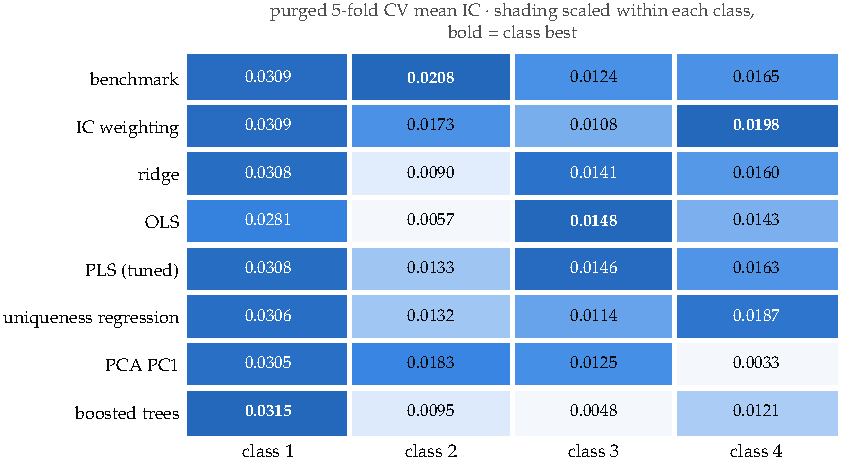
\includegraphics[width=0.66\textwidth]{fig_crossclass.pdf}
\caption{Purged 5-fold CV mean IC for every method on every class. Shading is scaled
within each class column (darker = higher IC on that class) and the bold entry marks the
class best. The benchmark is the robust anchor everywhere, supervision helps only where
the cluster is diffuse (class~4), and trees collapse on the three smaller or tighter
classes.}
\label{fig:crossclass}
\end{figure}

The sharper instrument is Figure~\ref{fig:preddim}: an out-of-fold PLS-$k$ sweep per class,
measuring how many predictive directions each cluster has, next to its eigen-spectrum
measuring variance directions. The two disagree in both directions, and the
disagreements are invisible to any unsupervised analysis.

\begin{itemize}
\item Class 4 looks multi-factor but predicts one-dimensionally. Variance is
      spread across many directions (PC1 only 30\%), yet everything predictive lies along
      the first supervised direction. IC weighting's class-4 edge is not about combining
      several predictive factors. It is about finding the one predictive direction
      when PC1 no longer points at it.
\item Class 3 is the reverse: two variance blocks, many predictive directions.
      Out-of-fold IC keeps rising to $k=6$. Later, low-variance directions carry real
      incremental information, which is why regression-style fits (OLS, small-$\lambda$
      GLS) top this class.
\end{itemize}

\begin{figure}[!tbp]
\centering
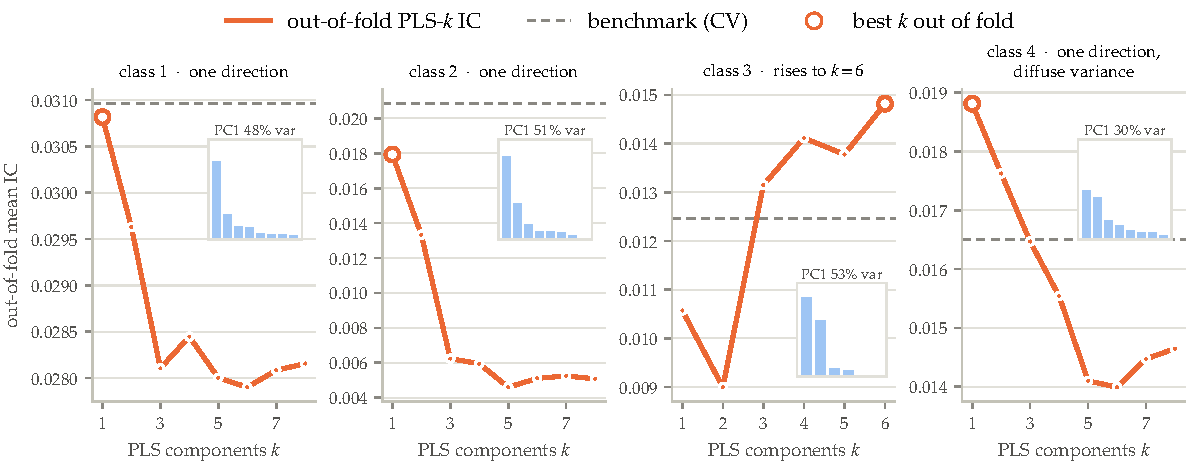
\includegraphics[width=0.94\textwidth]{fig_preddim.pdf}
\caption{Predictive dimension per class: out-of-fold PLS-$k$ IC (line, best $k$ circled;
the benchmark's CV IC dashed for reference) and the feature eigen-spectrum (inset
bars). Classes 1 and 2: one direction. Class 4: one predictive direction hiding in a
diffuse variance structure. Class 3: predictive content spread across many
low-variance directions.}
\label{fig:preddim}
\end{figure}

These profiles are the study's central diagnostic reading, and they dictated what to build
next. Class 4's profile says the valuable operation there is not estimating clever weights
but identifying which variants repeat one idea, so that the single predictive
direction stops being drowned by the most-duplicated definition: exactly deduplication, no
regression required. Class 3's profile says the opposite temptation (chase the extra
directions with a fitted $k$ or a GLS solve) is real but rests on one free parameter
estimated from a weak class, and Section~\ref{sec:holdout-retired} shows what honoring that
temptation costs when the fit is frozen. Classes 1 and 2 say: any sensible weighting works,
so spend the complexity budget elsewhere or not at all. One route satisfies all four
readings at once, cluster the redundancy away and weight the surviving ideas equally, and
that is the route the next section takes.

\subsection{Deduplication}
\label{sec:insample-cluster}

The cluster-then-weight family, cross-validated on all classes with paired out-of-fold
Newey--West tests against both anchors (the benchmark and IC weighting), delivers the
study's cleanest positive and negative findings.

\begin{enumerate}
\item Dedup with equal weights, cluster then count each idea once, is the only method that
      never loses to the benchmark anywhere, and the only one that ever significantly
      beats it. On class~4 it gains $+0.0028$ daily IC over the benchmark with
      Newey--West $t=2.26$, using no target information beyond sign bits. Supervised
      rivals post slightly larger point gains there ($+0.0033$/$+0.0036$) with lower
      significance ($t=1.82$/$1.63$): estimated weights add point-estimate gains and
      variance in roughly equal measure. The central premise is confirmed out of fold.
      The benchmark's flaw is duplication, not equal weighting, and fixing only
      duplication captures the achievable gain at zero supervision cost.
\item Supervision is a measurable tax wherever the cluster is one clean factor.
      On class~2 every target-using weighting (IC weighting, the uniqueness regression,
      and its tuned version) is significantly worse than the benchmark, with deficits of
      35 to 117 basis points of daily IC (1 bp $=$ 0.0001) at $t$ between $-2.4$ and
      $-2.9$. One predictive direction plus noisy daily ICs means estimated weights are
      noise around the equal-weight optimum: the forecast-combination puzzle, reproduced
      inside a single signal.
\item Adaptivity by search fails, and so does the soft prior. Letting inner validation
      pick the method per class is never terrible and never optimal. Model selection is itself an
      estimation problem: candidates differ by 0.002--0.004 against inner-slice noise an
      order larger. A tuned shrink-toward-equal-weights penalty never wins
      either. The hard version of the same prior (clustering) beats the soft version
      (a penalty), because it injects structure rather than another free parameter.
\item Nothing is hiding in the estimation window. Rolling and daily re-estimation
      (including literal daily PCA from each day's $\sim$500-name cross-section) only
      lose. The redundancy structure is time-stable, so trailing windows add estimation
      noise and remove nothing. Pool everything.
\end{enumerate}

Because the one significant win sits only just past the $2\sigma$ line, I also checked its
sensitivity to the concordance measure within the rank family: re-scoring the identical
out-of-fold signals under Kendall's $\tau$, which no single name can dominate, the class-4
win holds at $+0.0019$ with Newey--West $t = 2.29$, marginally stronger than under
Spearman, and every $t$ in the eight-row check moves by at most 0.04. Both measures are
rank-based by design (Section~\ref{sec:framework}). What the check establishes is that the
win is broad concordance across the cross-section rather than a handful of influential
names, not that the result is independent of the rank-based scope itself.

\subsection{The heterogeneity estimator as a detector}
\label{sec:insample-dl}

Section~\ref{sec:methods-dl}'s estimator was imported to make the equal-versus-IC-weights
decision by estimation rather than search, and it delivered as a \emph{detector}. Estimated
per class and per fold from training data alone, the heterogeneity parameter came back
$\hat\tau^2=0$ (to display precision) in all five folds on classes 1--3, prescribing full
pooling into equal weights, and $\hat\tau^2>0$ in all five folds on class~4, prescribing
that the IC differences be kept. That is precisely the supervision map Sections
\ref{sec:insample-map}--\ref{sec:insample-cluster} needed a battery of paired tests to
establish, recovered by one closed-form formula with nothing to tune. The estimator's
choices also paid directly. On class~2 the DL-weighted composite dodges the supervision
tax automatically and beats IC weighting significantly ($+0.0036$, $t=2.52$), and the
adaptive-weight variant of the dedup composite matched the per-class best method
everywhere with zero tuned weighting decisions.

Two caveats were recorded at the time, and both mattered later. First, the adaptive
variant's edges over the plain equal-weight form were never individually significant.
Second, detection and monetization are different claims: $\hat\tau^2>0$ says class-4
blocks truly differ in information content, but it does not guarantee that weights fitted
to those differences transfer forward. The blind hold-out confirmed exactly this gap
(Section~\ref{sec:holdout}), and the lesson, keep the detector and drop the tilt, became
the final method's form. We also tested a natural two-level extension, shrinking each
variant's IC toward its block mean rather than collapsing the block outright: offered any
pooling depth, the estimator chose full pooling in 19 of 20 class-folds. Within a
redundancy block, member ICs are statistically indistinguishable. The idea was not wrong,
it was already embedded in the method.

\subsection{What the trees contribute}
\label{sec:insample-trees}

XGBoost's one out-of-fold-verified edge on class~1 was not accuracy but trading behavior:
5-day IC retention of 0.72 against roughly 0.60 for the linear composites, a half-life of
11.1 days against 6.8, and the lowest 5-day factor turnover of any method. Depth-1
stumps, which cannot represent interactions, reproduce the full tree's entire profile,
and no construction on the linear composite does. The edge is therefore learned additive
per-feature response curves, extractable from the stump ensemble in closed form as 16
lookup tables (Figure~\ref{fig:shapes}). The curves are flat through mid-ranks, where
daily rank jitter lives, and respond only in the extreme tail, a slowly-changing state.
That is the turnover mechanism, and a two-compartment decay fit prices it: the share of
the signal decaying on the slow timescale rises from 0.29 for the linear composite to
0.54 for the shaped one. In effect the data redrew the ruler each variant is measured
with, and the ruler it drew ignores mid-pack shuffling and counts only depth into the
tail: the composite says the same thing it always said, it just stops changing its mind
over noise.

Grafting the shapes onto the dedup composite produced the study's most useful single
object. On class~1 the shaped composite reaches a half-life of 13.5 days, retention of
0.73, and turnover of 0.36 in-sample, out-trading the tree that taught it the shapes, at
the linear ceiling's accuracy. On classes 2--4, applying shapes unconditionally is
somewhere between pointless and disastrous (class~2: $-0.0180$, $t=-2.97$). Six hundred
stumps on 1{,}500 days repeats the tree collapse of Section~\ref{sec:insample-map},
which is exactly why shapes only enter behind the evidence gate of
Section~\ref{sec:methods-shapes}. The gate adopts class~1 alone.

\begin{figure}[!tbp]
\centering
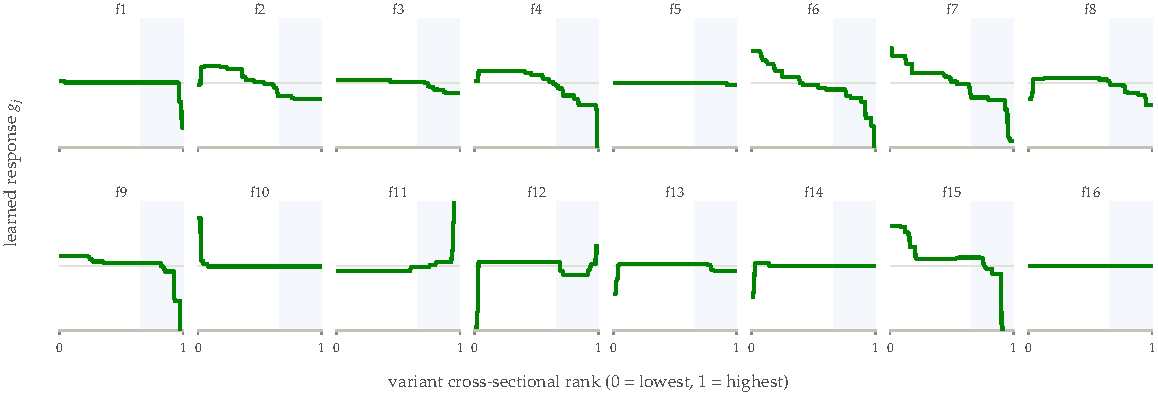
\includegraphics[width=0.9\textwidth]{fig_shapes.pdf}
\caption{The learned per-feature transforms, extracted exactly from the depth-1 ensemble
(each panel on its own vertical scale; the shaded band is the top third of ranks). The
curves are flat through the middle of each variant's rank range and respond sharply in the
extreme tail: 75\% of total response movement lives in the top third, 6\% in the middle.
The model reads class~1 as a tail-depth detector, and the production model is 16 lookup
tables, no tree library required.}
\label{fig:shapes}
\end{figure}

\FloatBarrier
\subsection{Stress tests}
\label{sec:insample-stress}

Before the hold-out, I attacked the dedup composite from every direction I was able to
think of, as well as those raised in sponsor meetings. Two examples:

\begin{itemize}
\item Partition construction. Five linkages, an IC-profile similarity, a top-down
      divisive tree, and a random placebo, all at matched block count: the partition
      matters only on class~4, where the anchor tree wins and the placebo collapses
      ($-0.0025$). It is irrelevant by construction wherever $\hat\tau^2=0$ forces equal
      block weights.
\item Tuned merge threshold. Per-fold inner-validation tuning of $\rho$ over a
      wide grid confirms 0.7 (class~4: five folds of five), picks a stable neighbor that
      buys nothing (class~1: 0.8 in five of five, $+0.0006$, not significant), or
      whipsaws unstably (classes 2--3) and costs money. The sensitivity table's best cell
      (class~2 at $\rho=0.8$, ten basis points above the selected value) is not ex-ante
      selectable: leak-free tuning delivered 0.0208, not 0.0226. The gap between the best
      cell in a sensitivity table and what tuning actually delivers is this study's
      recurring look-ahead lesson.
\end{itemize}

The test that ended up anchoring my confidence came from perturbing the feature set
itself. The premise of the whole project is that the exact list of variants a class
contains is arbitrary at the margin: a team could easily have delivered 12 of these 16
variants rather than all 16, so a composition method must not depend on the exact list it
happened to receive. I therefore re-ran the full purged CV on 80 randomly reduced feature
sets, 20 per class, each formed by dropping roughly 25\% of that class's variants at
random, and scored every method on every subset (Figure~\ref{fig:menus}). The result is
the study's clearest separation. The dedup composite ranks top-2 in mean rank on classes
1--3 and mid-pack on class~4 (behind the two IC-tilted arms), and its worst case is the
shallowest of anything tried, jointly with its adaptive-weight sibling
(Figure~\ref{fig:nutshell}, panel~B). Every rival craters somewhere: the benchmark is
last on 17 of 20 class-4 subsets with the lowest floor there, since dropping the right
variants leaves its duplication bias nothing to hide behind; tuned uniqueness collapses on class~2
(its worst subsets sit at roughly 40\% of the benchmark's IC), and the GLS edge on
class~3 inverts under perturbation. Robustness of this kind is invisible in any single
full-set comparison, and it is the property a desk actually needs: the composite never
needs to know which class, or which subset of a class, it is running on. That property,
not any mean edge, is why the multiplicity verdict of Section~\ref{sec:referee} (``the
floor, not the mean'') matches the method's natural defense.

\begin{figure}[!b]
\centering
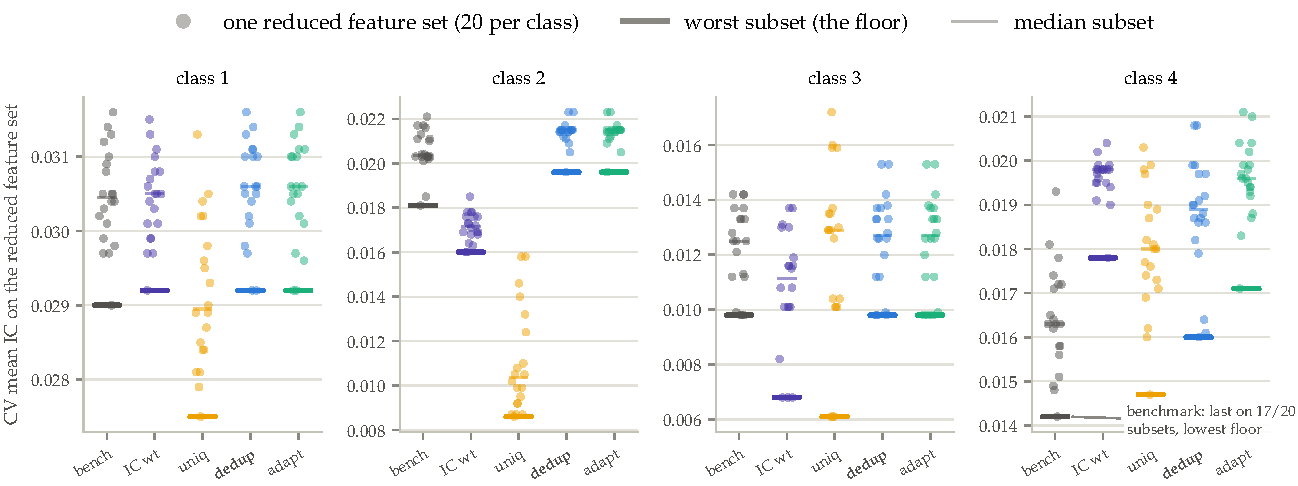
\includegraphics[width=0.99\textwidth]{fig_menus.pdf}
\caption{The feature-subset stress test: 80 randomly reduced feature sets (20 per class,
$\sim$25\% of variants removed, full purged CV re-run per subset). Each dot is one
reduced subset's CV mean IC for one method; colors identify methods, consistent with the
other figures. The heavy tick is each method's worst subset, its floor, and the thin tick
the median. The dedup composite (``dedup'') holds the highest or joint-highest floor on
classes 1--3 and the joint-shallowest worst-case shortfall overall. The benchmark is last
on 17 of 20 class-4 subsets with the lowest floor there, and tuned uniqueness craters on
classes 2 and 3.}
\label{fig:menus}
\end{figure}

% =====================================================================
\FloatBarrier
\section{The blind hold-out}
\label{sec:holdout}

\subsection{Protocol}

The hold-out arrived after the in-sample study was complete: the immediately following
2{,}195 calendar-indexed trading days for every class ($\sim$2{,}180 scoreable days,
$\sim$430 names per day). The protocol is strict freeze. Every parameter (feature signs,
IC weights, tuned $\lambda$ and $\rho$, the clustering, the adaptive block weights, the
XGBoost model, the stump shapes and the gate decision, even standardization constants) was
estimated once on in-sample data and applied unchanged. Nothing is fit, tuned, or selected
on the hold-out. One further lock was applied: after the final in-sample review confirmed
that tuning $\rho$ yielded negative results and that no universal fixed $\rho$
significantly beats 0.7, we fixed it at 0.7. The textbook regressions (OLS, ridge, lasso)
were retired in-sample due to their unpromising results and not frozen for hold-out
scoring. The tuned uniqueness arm stands in place for the regression family below.

\subsection{Results}
\label{sec:holdout-results}

\begin{figure}[!tb]
\centering
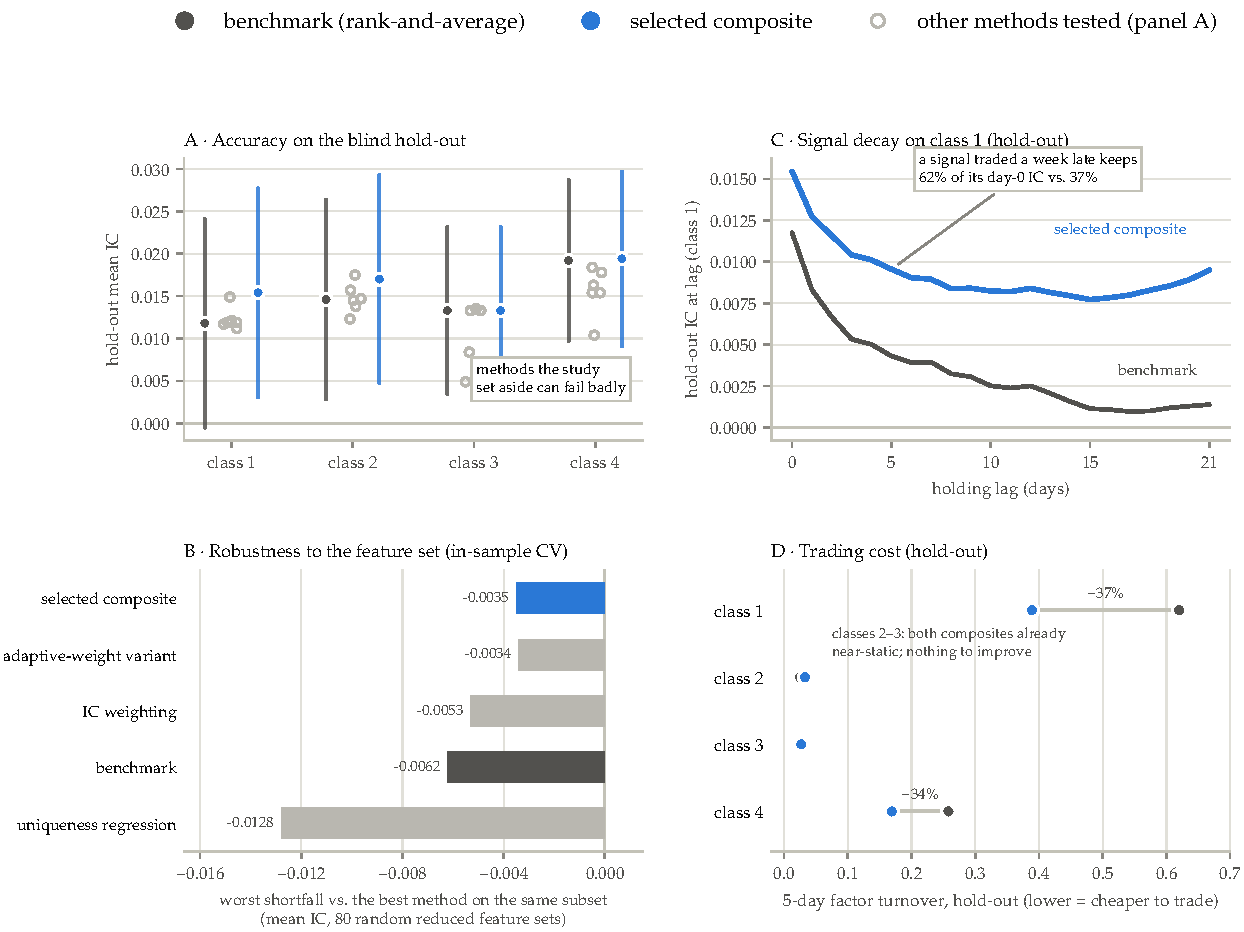
\includegraphics[width=0.98\textwidth]{fig_nutshell.pdf}
\caption{The study in one figure. Throughout, gray marks the benchmark, blue the selected
composite (on class~1 this includes the learned feature shapes), and small open gray
circles the other frozen methods. (A)~Hold-out mean IC per class with 95\% Newey--West
confidence whiskers: the selected composite matches or exceeds the benchmark everywhere,
and the low gray circles on classes 3--4 show how badly the discarded methods (PCA, tuned
PLS, boosted trees) can fail. (B)~The one in-sample panel: across 80 randomly reduced
feature sets (Section~\ref{sec:insample-stress}), each bar is a method's worst shortfall
against the best method on the same subset, and the selected composite's worst case is
the shallowest. This test is pre-freeze by construction, since re-running method
selection on the hold-out would contaminate it. (C)~Hold-out IC by holding lag on
class~1, the class where the composites differ most: the selected composite starts higher
and decays far more slowly. (D)~Five-day factor turnover per class: lower for the
selected composite where the two composites differ (classes 1 and 4), unchanged where
they coincide.}
\label{fig:nutshell}
\end{figure}

Figure~\ref{fig:forest} is the scorecard and Figure~\ref{fig:nutshell} the study in one
figure, and the full numeric table is Appendix~\ref{app:scorecard}. Three headlines order the
results. First, the signals are real out of sample: classes 2--4 are significantly
positive under strict freeze, with Newey--West $t$ between 2.4 and 3.9 for the benchmark
and dedup composites. Second, the accuracy claim replicates exactly as stated, which is
to say at zero: the dedup composite minus the benchmark is approximately zero everywhere
(max $|t|=1.1$ for the linear form, 1.3 including the shaped class-1 arm), while the
composite matches or exceeds the benchmark on every class. Third, everything the study
had flagged as fragile is precisely what failed. Three results deserve their own
paragraphs.

\begin{figure}[!tb]
\centering
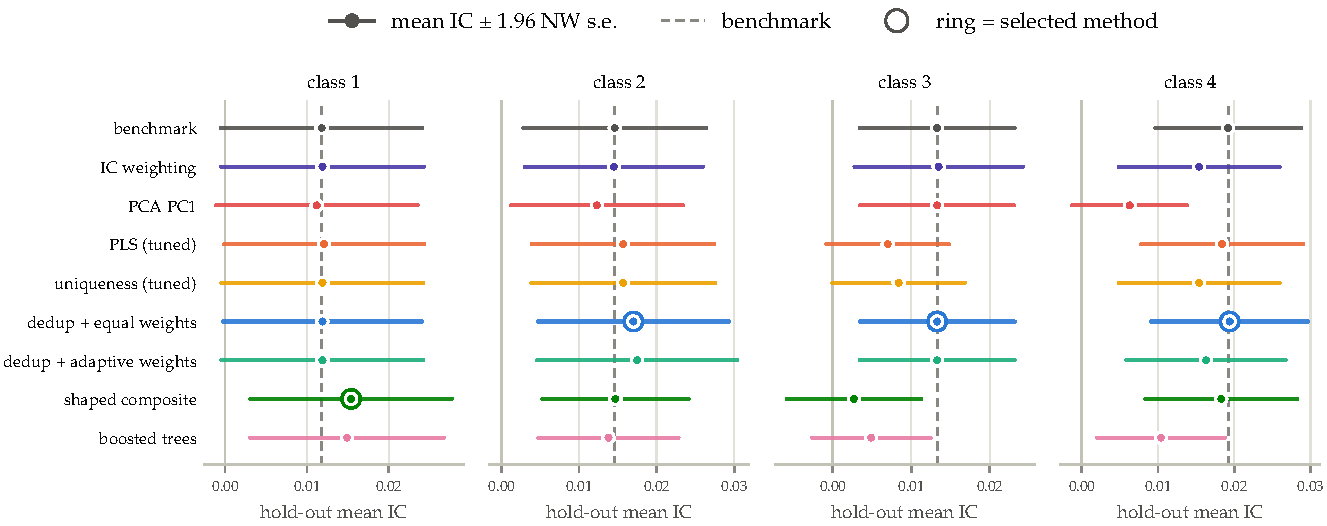
\includegraphics[width=0.94\textwidth]{fig_forest.pdf}
\caption{The frozen methods on the blind hold-out ($\sim$2{,}180 unseen days per class):
mean daily rank IC with $\pm1.96$ Newey--West standard errors. The dashed line is the
benchmark's level, and the ring marks the method selected for each class. The selected
composite matches or beats the benchmark on every class. Classes 3 and 4 realized above
their in-sample CV level, a period effect at the year scale (Figure~\ref{fig:rolling}).
The two instructive failures are visible at a glance: PCA collapses on the multi-factor
class~4, and tuned PLS and the shaped arm both break on class~3.}
\label{fig:forest}
\end{figure}

\paragraph{Class 1 is the alpha-decay lesson.} Its linear composites lost two-thirds of
their IC (0.031 $\to$ 0.0119, $t\approx1.9$), yet the drift diagnostic shows the
redundancy structure barely moved. The correlation matrix's Frobenius drift is 0.22, in
line with the other classes, not one of 16 variants flips IC sign, and all shrink
uniformly 50--70\%. The correlation matrix is stable; the signal level decayed.
Figure~\ref{fig:rolling} shows how: the rolling one-year IC sits near, mostly slightly
below, the in-sample level for most of the eight-year window and breaks downward in the
final year, while classes 2--4 cycle around positive means. Nothing re-weightable was
lost. A rolling re-estimation arm (quarterly refits on an expanding window) recovers
exactly nothing on class~1, because there is nothing stale to refresh. The operational
moral for any frozen composite is to monitor the level, not just the structure, because
alpha decay cannot be recovered by re-estimation.

\begin{figure}[!tb]
\centering
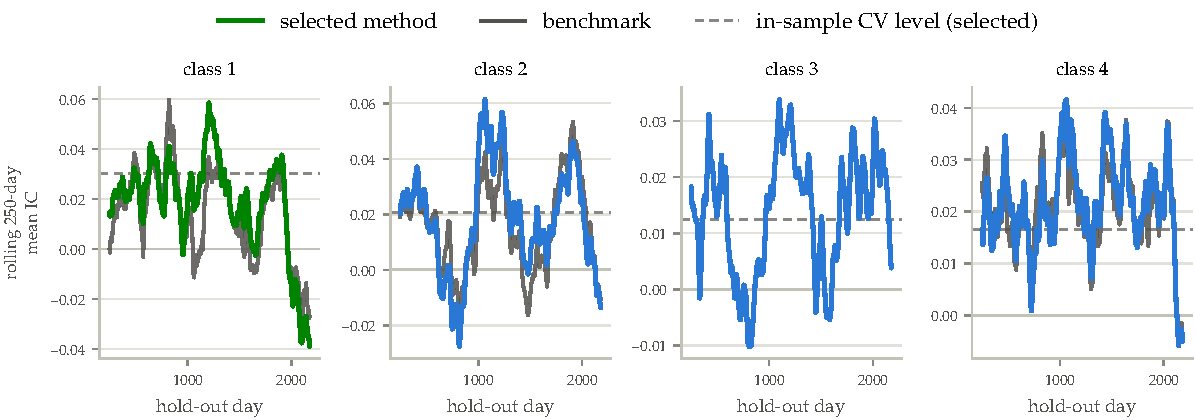
\includegraphics[width=0.94\textwidth]{fig_rolling.pdf}
\caption{The hold-out IC through time: rolling 250-day mean IC of the selected method
(green) against the benchmark (gray), per class, with the selected method's in-sample CV
level dashed for reference. Class~1's loss concentrates in the final year of the window,
while classes 2--4 cycle with year-scale swings around positive means.}
\label{fig:rolling}
\end{figure}

\paragraph{The shaped composite is the class-1 method that survives.} Every linear
composite sits at $t\approx1.9$ on class~1. The shaped composite is the only
linear-family composite still significant there, and against the one other survivor, the
tree that taught it the shapes, it matches on accuracy and wins on every tradeability
axis:

\begin{center}
\small
\begin{tabular}{lccccc}
\toprule
class 1, hold-out & mean IC & NW $t$ & 5-day retention & half-life & 5-day turnover \\
\midrule
shaped composite & 0.0154 & 2.45 & 0.62 & 15.0d & 0.39 \\
boosted trees & 0.0149 & 2.47 & 0.54 & 7.0d & 0.57 \\
linear dedup / benchmark & 0.0119 & 1.9 & 0.37 & 2.6d & $\sim$0.6 \\
\bottomrule
\end{tabular}
\end{center}

\noindent The shaped-minus-linear IC gap ($+0.0035$, $t=1.3$) is not itself significant.
The case for shapes is IC parity plus the trading profile, priced jointly in
Section~\ref{sec:referee}. The pre-specified sign-aligned refinement of the shaped arm
(flip each block member by the sign of its train IC before averaging) ties the original
everywhere (0.0155 vs.\ 0.0154): the tidy-up was safe, not material.

\paragraph{The adaptive tilt is the casualty.} The adaptive-weight variant trails plain
equal weights by $-0.0031$ ($t=-3.4$) on class~4, the one class where the weights differ.
Quarterly re-estimation lifts the tilt only to 0.0182, still below frozen equal weights
at 0.0194: tilt plus maintenance loses to equal weights frozen forever. The detector
stays and the tilt goes. From here on the selected composite means the equal-weights
form, with the adaptive variant demoted to a candidate the blind test retired.

\subsection{PCA and PLS out of sample}
\label{sec:holdout-retired}

Because the in-sample study retired PCA and tuned PLS on in-sample evidence alone, both
were frozen post hoc under the identical protocol and scored: a test of the retirement
decisions themselves on data neither method ever saw (Figure~\ref{fig:retired}).

For PCA, retirement is confirmed. Where a cluster is near-one-factor, PC1 essentially is
the average and adds nothing (class~3: 0.0133 vs.\ 0.0133, the curves coincide). On the
one multi-factor class it keeps a third of the benchmark's IC (0.0063 vs.\ 0.0192) while
trading more and decaying faster. As a four-class package it posts the study's only
$|t|>3$ pooled result, a deficit (Section~\ref{sec:referee}). Out of sample as in
sample, variance is the wrong objective.

PLS is the sharpest exhibit of the study's recurring pattern. Where the tuner froze
$k=1$ (classes 1 and 4), one-component PLS approximately equals IC weighting, as the
algebra requires, and on class~2 its frozen $k=2$ is the one tuning win ($+0.0011$, not
significant). But on class~3 the tuner froze $k=6$, a defensible choice given that the
in-sample out-of-fold sweep really does rise with $k$, and the hold-out falls with $k$
instead: 0.0070 against 0.0135 at $k=1$. One leak-free inner-validation decision on one
free parameter cost the class half its IC. Supervision that wins the inner split does not
survive the freeze. This is the same lesson as the tuned $\rho$ and the monetized
$\tau^2$: when estimation is introduced, much of the intended benefit is lost to noise.

\begin{figure}[!tb]
\centering
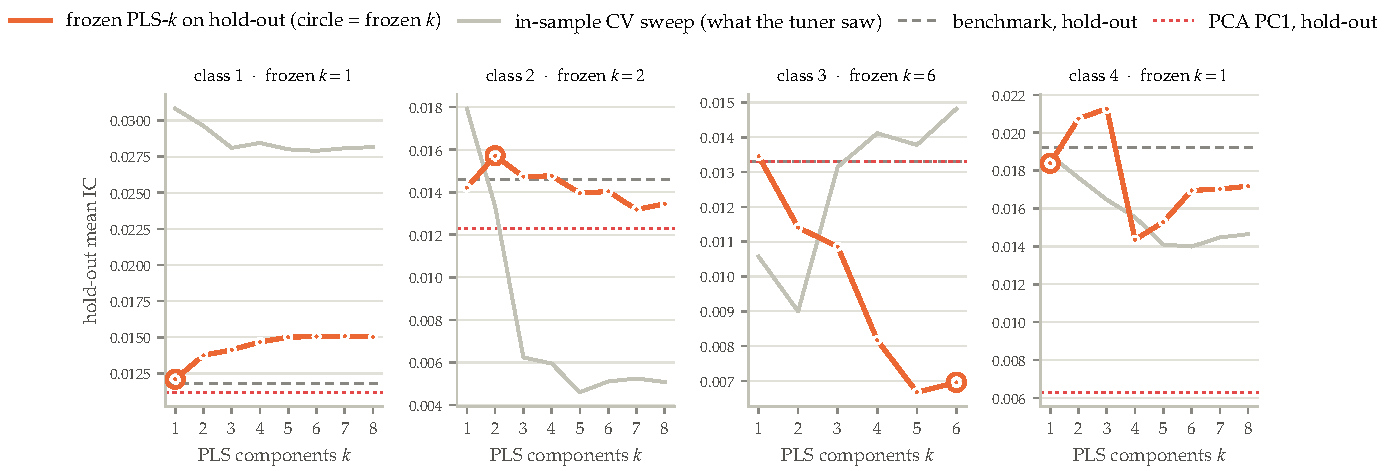
\includegraphics[width=0.94\textwidth]{fig_retired.pdf}
\caption{The frozen PLS-$k$ sweep on the hold-out, per class. The orange line is the
frozen PLS composite's hold-out IC as a function of the number of components $k$, the
circle marks the $k$ chosen on in-sample inner validation and then frozen, the gray line
is the in-sample CV sweep the tuner saw, and the dashed lines are the frozen benchmark
and PCA PC1 hold-out levels for reference. On class~3 the in-sample sweep rises to $k=6$
while the hold-out falls with $k$ instead: the inner-validation choice halves the class's
IC. Because $k$ is estimated in sample, estimation noise means the out-of-sample
optimum can sit at a starkly different $k$; the intended benefit is lost in the act of
estimating.}
\label{fig:retired}
\end{figure}

% =====================================================================
\FloatBarrier
\section{Statistical checks}
\label{sec:referee}

\subsection{Multiplicity correction}
\label{sec:referee-mult}

The study ran 56 paired ``does $X$ beat the benchmark?'' comparisons, all on the
purged-CV out-of-fold record (12 methods $\times$ 4 classes, plus the retired PCA and
PLS; hold-out differences are reported separately in Section~\ref{sec:holdout}). Seven
clear $|t|>2$ nominally: six negative and one positive (the dedup composite's class-4
win, $t=2.26$). Following \citet{harvey2016}, I correct the whole family
(Figure~\ref{fig:mult}). Zero tests survive Holm at 5\%, Benjamini--Hochberg at 5\%, or
the dependence-aware Westfall--Young max-$T$ (block bootstrap, whose 95\% bar sits at
$|t|\approx3.75$; the win's adjusted $p\approx0.66$). At the looser BH 10\%
false-discovery rate, exactly two results survive, both negative: PCA on class~4
($-0.0132$, $t=-3.11$) and tuned uniqueness on class~2 ($-0.0117$, $t=-2.93$). The only
comparisons that retain any post-correction standing in the whole study are negative
results.

\begin{figure}[!tbp]
\centering
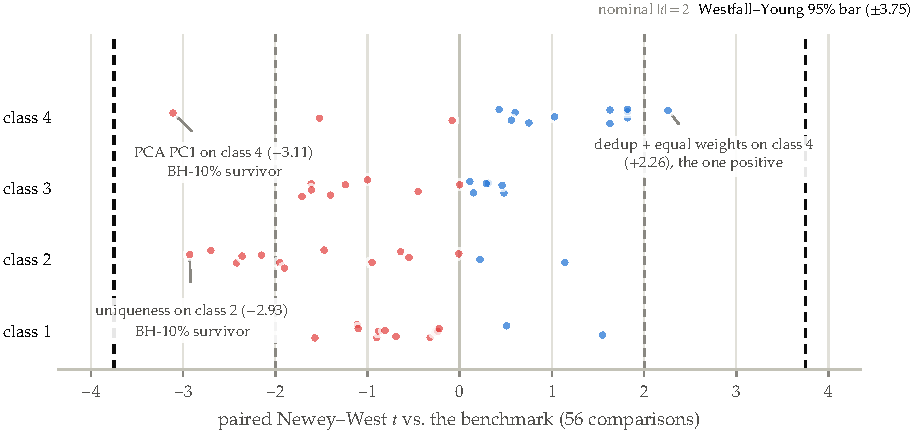
\includegraphics[width=0.78\textwidth]{fig_mult.pdf}
\caption{Every paired method-versus-benchmark $t$-statistic in the study (the in-sample
purged-CV family), one dot per method and class, blue for positive and red for negative.
The inner dashed lines mark nominal $|t|=2$, which flags seven comparisons; the outer
dashed lines mark the dependence-aware Westfall--Young 95\% max-$T$ bar ($\pm3.75$),
which flags none. The two survivors at the looser BH-10\% rate are both negative
results.}
\label{fig:mult}
\end{figure}

This re-frames the study. No positive paired comparison here, including our own headline
win, should be quoted as significant on its own. The defensible claim shifts to where the
stress tests had already placed it, the floor rather than the mean, which multiplicity
correction does not touch. The negative census, meanwhile, has teeth: do not chase
variance on a multi-factor cluster, and do not supervise a one-factor cluster, is the
closest thing to a certified finding this analysis produced. The test has power, since it
flags the known pathologies at BH 10\%, so the null results elsewhere reflect an
absence of effect rather than an absence of power.

\subsection{Robustness of the heterogeneity detection}
\label{sec:referee-tau}

DerSimonian--Laird is known to be noisy at small $k$. Re-estimating the method's one
data-driven decision with the Paule--Mandel and REML estimators reproduces the $\tau^2$
map, zero on classes 1--3 and positive on class~4, at the frozen full-sample level, and
all three estimators find $\hat\tau^2>0$ in every one of class~4's five CV folds. The
detection is estimator-robust. But frozen on the class-4 hold-out, the three tilts all
land between 0.0163 and 0.0166 while equal weights score 0.0194: whatever $\tau^2$
correctly measured about in-sample heterogeneity, the weights it prescribes did not carry
forward. The Hartung--Knapp intervals explain the failure in one number. With $k=2$
blocks (class~3) the 95\% interval on the pooled block IC is $[-0.016, +0.036]$. At these
block counts the estimator can detect heterogeneity but cannot support differential
weights. Detection is robust, monetization fails, and the method keeps $\tau^2$ as a
diagnostic flag with equal weights as the action.

\subsection{Shape stability across feature subsets}
\label{sec:referee-shapes}

The class-1 shape edge was learned on the 16 variants the class happened to contain, so I
re-learned it on each of the twenty reduced feature subsets of
Section~\ref{sec:insample-stress} (per-fold stump refits in CV, then freeze-forward
scoring on the hold-out). In sample, the shaped composite's CV cost is a rounding error:
mean $-0.0002$, with zero significant losses in 20 subsets. Out of sample, the frozen
shaped arm beats the frozen linear arm on IC on 18 of 20 subsets (mean $+0.0021$), trades
less on 17 of 20, retains 0.61 of its IC at lag 5 against 0.39, and wins the weekly
criterion below on 20 of 20. The gate, replayed per subset, adopts on 19 of 20. Its one
refusal cost $+0.0003$ on the single subset where the shaped arm did churn more out of
sample, so the screen caught a real defect cheaply. An edge that survives twenty random
re-drawings of its inputs, on unseen data, in level and profile, is a property of the
class, not of the exact feature list.

\subsection{A weekly rebalancing criterion}
\label{sec:referee-combo}

The metrics so far price accuracy and trading behavior separately, but a real book earns
them jointly, so the last check prices them together. Ultramarin's holding horizon is
mid-to-low frequency, in the neighborhood of days to weeks, so we take weekly
rebalancing as the measurement criterion. Between rebalances such a book trades on a
signal that is between zero and five days stale, so the IC it earns is approximated by
the average of the lag-0 and lag-5 daily ICs. That average is the criterion used here:
it captures level and decay in one number and, as a daily series, supports the same
paired Newey--West testing as everything else. Against the benchmark, the only material per-class term is shapes on
class~1: $+0.0047$ per day ($t=1.6$), a 59\% relative improvement (0.0127 vs.\ 0.0080),
earned because the benchmark keeps 37\% of its IC at lag 5 while the shaped arm keeps
65\%. Everything else is noise-level. Pooling day-by-day across classes gives
Table~\ref{tab:combo}.

\begin{table}[!htbp]
\centering
\small
\caption{The weekly level-plus-decay criterion, pooled across classes, paired against the
benchmark on the hold-out. Each row is one four-class package: which composite serves
each class. The retired references calibrate the scale: the criterion can flag a bad
package at $t=-3$, so the selected package's $+1.72$ is competing against a real zero,
not against a test with no power.}
\label{tab:combo}
\begin{tabular}{lcc}
\toprule
four-class package & weekly-criterion edge vs.\ benchmark (per day) & NW $t$ \\
\midrule
shaped c1 + dedup eq.\ c2--4 (selected) & $+0.0019$ & $+1.72$ \\
shaped c1 + dedup adaptive c2--4 & $+0.0013$ & $+1.02$ \\
dedup equal weights everywhere & $+0.0007$ & $+1.05$ \\
dedup adaptive weights everywhere & $+0.0001$ & $+0.09$ \\
\emph{PCA PC1 everywhere (retired reference)} & $-0.0039$ & $-3.07$ \\
\emph{PLS tuned everywhere (retired reference)} & $-0.0013$ & $-1.20$ \\
\bottomrule
\end{tabular}
\end{table}

\enlargethispage{\baselineskip}%
Two labels belong on this number. The $t$ of 1.72 is suggestive, not certified, and the
package combination is post hoc, although its components were pre-specified. Turnover
sits on top of the criterion: the winning package trades at roughly 60\% of the
benchmark's turnover on class~1 and roughly 35\% lower on class~4. What makes the number
credible is its consistency. The same ordering holds on every class where anything
differs, on 20 of 20 class-1 feature subsets, and under every aggregation tried.
Figure~\ref{fig:dominance} is the graphical form: the selected package's hold-out IC is
at or above the benchmark's at every holding lag on every class, and on the two classes
where the method changed anything (1 and 4) the edge grows with the holding period.

\begin{figure}[!b]
\centering
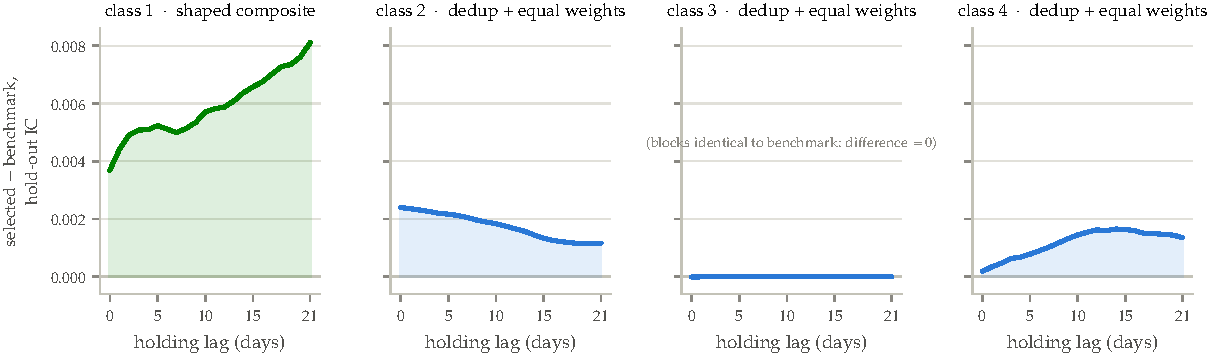
\includegraphics[width=0.9\textwidth]{fig_dominance.pdf}
\caption{Selected composite minus benchmark, hold-out IC at every holding lag, per class,
on one vertical scale throughout; this is the per-class expansion of the weekly
criterion. The shaded difference is at or above zero everywhere:
no holding horizon, on any class, favored the benchmark over the hold-out period. On
class~3 the selected composite's blocks coincide with the benchmark, so the difference is
identically zero.}
\label{fig:dominance}
\end{figure}

% =====================================================================
\FloatBarrier
\section{The selected composite methodology}
\label{sec:recipe}

\begin{figure}[!tbp]
\centering
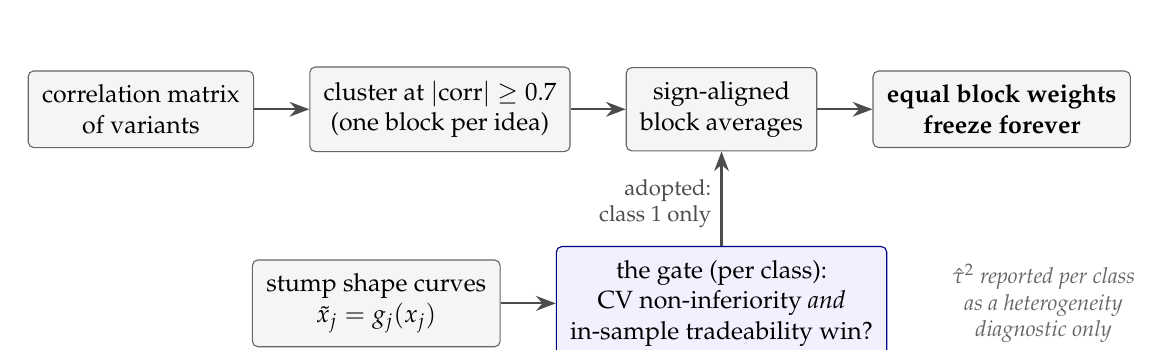
\begin{tikzpicture}[
  node distance=5mm and 7mm,
  box/.style={rectangle,rounded corners=2pt,draw=black!60,fill=black!4,align=center,
              font=\small,inner sep=5pt,minimum height=9mm},
  gate/.style={rectangle,rounded corners=2pt,draw=blue!50!black,fill=blue!6,align=center,
              font=\small,inner sep=5pt,minimum height=9mm},
  note/.style={font=\footnotesize\itshape,text=black!60,align=center},
  arr/.style={-{Stealth[length=2.5mm]},thick,black!70}
]
\node[box] (corr) {correlation matrix\\of variants};
\node[box,right=of corr] (clust) {cluster at $|\mathrm{corr}|\ge0.7$\\(one block per idea)};
\node[box,right=of clust] (avg) {sign-aligned\\block averages};
\node[box,right=of avg] (eq) {\textbf{equal block weights}\\\textbf{freeze forever}};
\node[gate,below=12mm of avg] (gatebox) {the gate (per class):\\CV non-inferiority \emph{and}\\in-sample tradeability win?};
\node[box,left=of gatebox] (shapes) {stump shape curves\\$\tilde{x}_j=g_j(x_j)$};
\node[note,anchor=west] (diag) at ([xshift=7mm]gatebox.east) {$\hat\tau^2$ reported per class\\as a heterogeneity\\diagnostic only};
\draw[arr] (corr) -- (clust);
\draw[arr] (clust) -- (avg);
\draw[arr] (avg) -- (eq);
\draw[arr] (shapes) -- (gatebox);
\draw[arr] (gatebox) -- node[left,font=\footnotesize,align=right,pos=0.45] {adopted:\\class 1 only~} (avg);
\end{tikzpicture}
\caption{The selected composite. Variants are clustered into idea-level blocks, averaged
within blocks, and the blocks weighted equally, with all parameters frozen. The gate is
the one data-driven decision point: learned feature shapes enter only where they pass the
two-stage in-sample bar of Section~\ref{sec:methods-shapes}, which happened on class~1
alone. There are no tuned hyperparameters and nothing on a re-estimation schedule.}
\label{fig:pipeline}
\end{figure}

The final specification (Figure~\ref{fig:pipeline}), with the evidence for each choice:

\begin{enumerate}
\item Group the duplicates. Cluster variants on $1-|\mathrm{corr}|$ (average
      linkage); variants more than 70\% correlated in absolute value merge into one block,
      so the same idea implemented several times gets one vote. The threshold is fixed
      forever: tuning was offered a wide grid twice and could not beat it, and the
      value has a structure-free meaning (shared variance $\approx$ half).
\item Average within blocks. Flip any variant whose train IC is negative, then
      simply average each block's members. A handful of idea-level signals replaces 6--20
      redundant variants.
\item Weight the ideas equally and freeze. The random-effects tilt
      detected real heterogeneity where blocks truly differed, confirmed by three
      estimators, but acting on it lost to frozen equal weights on the blind
      hold-out, and quarterly re-estimation only partially repaired that self-inflicted
      loss. Equal block weights match or beat the tilt everywhere, frozen, with no refit
      infrastructure.
      $\hat\tau^2$ stays in the pipeline as a diagnostic, a flag that a class is
      multi-factor and deserves attention, not as weights.
\item Shapes, only where the evidence clears the bar. Variants may first pass
      through their learned response curves (sign-aligned form), but only where the gate
      says so: empirically class~1 alone. On that class the shaped composite is the best
      method on the hold-out at roughly 60\% of the linear form's turnover, and the only
      composite in the linear family still significant there.
\end{enumerate}

\begin{table}[!htbp]
\centering
\small
\caption{The selected composite per class, with its blind hold-out scorecard. Classes
2--4 are the dedup-and-equal-weight rows throughout (retention and turnover recomputed
from the stored hold-out curves). Class~1 shows the shaped blind-test record; the
selected sign-aligned form is statistically identical (IC 0.0155, $t=2.44$, retention
0.65, turnover 0.37).}
\label{tab:ship}
\begin{tabular}{llccccc}
\toprule
class & composite & mean IC & NW $t$ & 5-day ret. & 5-day turn. & hit rate \\
\midrule
1 & shaped $\to$ dedup $\to$ equal blocks & 0.0154 & 2.45 & 0.62 & 0.39 & 0.57 \\
2 & raw $\to$ dedup $\to$ equal blocks & 0.0170 & 2.71 & 0.94 & 0.03 & 0.60 \\
3 & raw $\to$ dedup $\to$ equal blocks & 0.0133 & 2.64 & 0.97 & 0.03 & 0.60 \\
4 & raw $\to$ dedup $\to$ equal blocks & 0.0194 & 3.69 & 0.89 & 0.17 & 0.62 \\
\bottomrule
\end{tabular}
\end{table}

In one sentence: \emph{count each idea once, weight ideas equally, learn feature shapes
only where the evidence is strong, and freeze everything.} Its virtue is not extra IC.
After multiplicity accounting, nothing beats the benchmark on IC. Its virtue is that on
the level-plus-decay criterion a real book earns, it is consistently ahead
($+0.0019$ per day pooled, $t=1.7$, suggestive rather than certified, at 35--40\% lower
turnover where turnover matters), it has the joint-shallowest worst case of anything
tried, it is fully mechanical, and every moving part carries the test that justifies it.

Equally important is what the composite deliberately leaves out, because each exclusion
carries a documented failure: IC weighting (significantly hurts one-factor clusters),
GLS and uniqueness solves (the class-3 edge inverted out of sample), the adaptive tilt
($-0.0031$ frozen), scheduled re-estimation (repairs only the tilt's own damage), boosted
trees off class~1 (27--61\% IC collapse), tuned merge thresholds and search-based method
selection (whipsaw), and PCA (one-third of the benchmark's IC on the class where it
matters). A desk that adopted the ``obvious'' improvements without this discipline would
end up strictly worse than one deploying plain rank-and-average.

% =====================================================================
\FloatBarrier
\section{Discussion}
\label{sec:discussion}

Four anonymized classes cannot certify a universal rule; that is a sample of four. What
the study can hand Ultramarin is a set of cheap, mechanical diagnostics with a measured
track record, a map from diagnostic readings to actions, and a list of ideas that need
exactly the resources we did not have. This section is addressed to readers who know
what classes 1--4 actually are.

\subsection{A playbook for a new feature class}
\label{sec:discussion-playbook}

Everything below is computable from a new class's training panel in minutes, before any
composite is deployed.

\begin{enumerate}
\item PC1 variance share and the redundancy dendrogram
      (Section~\ref{sec:data}). Above $\sim$0.45 with clean blocks: equal weighting will
      saturate the class, and the composite without shapes is likely already optimal. A
      diffuse spectrum (class-4-like, PC1 $\sim$0.3): the partition now matters, so
      inspect the dendrogram, and expect the plain benchmark to be the casualty (last on
      17 of 20 class-4 feature subsets, with the lowest floor).
\item The out-of-fold PLS-$k$ sweep (Figure~\ref{fig:preddim}). One peak at
      $k=1$: any sensible weighting works, so spend effort elsewhere. Rising past $k\ge3$
      (class-3-like): the class carries real multi-directional signal that block
      averaging partially destroys, but our evidence says do not chase it with a frozen
      tuned $k$ or a GLS fit (both inverted out of sample). Treat it as a research flag,
      not a production decision, until several such classes accumulate.
\item $\hat\tau^2$ across blocks, under all three estimators
      (Section~\ref{sec:methods-dl}). $\hat\tau^2=0$: equal weights are
      optimal-in-family, not merely safe; walk away. $\hat\tau^2>0$ under all three:
      the blocks truly differ. On our data acting on that signal failed ($k\le9$ blocks
      cannot support estimated weights, and the Hartung--Knapp intervals say why), but
      the detection was flawless, 5 of 5 folds and 3 of 3 estimators. On a future class
      with many more blocks ($k\ge20$) or externally-known block identities, the tilt
      deserves a fresh trial: not fruitful to act on here, demonstrably correct as a
      detector.
\item The gate for shapes (Section~\ref{sec:methods-shapes}). Run the stump fit
      and the two-stage bar. Its measured operating characteristics: 19 of 20 correct
      adoptions across feature subsets, one benign refusal, one prevented out-of-sample
      blow-up (class~3; the class-2 refusal rests on decisive in-sample evidence), and
      refusals on classes 2 and 4 that cost the selected composite nothing on the
      hold-out. That is the conservative failure mode you want in production.
\item After deployment, monitor the level, not just the structure. Class~1's
      correlation matrix was rock-stable while its alpha halved, so a structural drift
      alarm alone would have missed the one failure that actually occurred
      (Figure~\ref{fig:rolling}). Track the trailing-year mean IC against the in-sample
      rolling distribution and alarm below its 5th percentile, treating structural drift
      as a separate, second alarm.
\end{enumerate}

\subsection{What we would explore with Ultramarin's resources}
\label{sec:discussion-future}

\begin{itemize}
\item Rolling windows and re-estimation, per future class. On our four classes
      rolling and scheduled re-estimation bought nothing, and the reason is diagnostic
      rather than universal. The composite has no weights to re-estimate, but it does
      have estimated structure: the clustering, the sign bits, the shape curves, and the
      gate decision. Our classes were structurally stable (hold-out correlation-matrix
      Frobenius drift between 0.16 and 0.42, unrelated to where performance fell), so
      refits had nothing to fix. Class~1's decline was alpha decay, which no
      re-estimation can recover, and the only rolling win anywhere ($+0.0019$, $t=3.4$,
      on class~4) merely repaired the retired tilt's own frozen-weight damage. A future
      class could differ, so this must be re-examined per class, and the playbook's
      drift diagnostics are the instruments that decide. Structural drift says re-derive
      the clustering and signs, which is safe because the re-derived object is still an
      equal-weighted partition with nothing continuous to overfit. Level decay says
      retire or de-weight, not refit.
\item Cross-class composition. Our mandate was within-class, but the four selected
      composites are themselves four correlated, noisy signals: exactly the structure
      this study composes. The natural next study runs the identical method one level up
      (dedup-then-equal-weight across class composites, $\tau^2$ as the diagnostic),
      where block identities are known and economically meaningful.
\item Real class identities. Every diagnostic here was run blind. Knowing the theme
      behind a class (momentum, quality, and so on) converts the per-class map from
      correlation into interpretation: whether uniform alpha decay of the class-1 kind
      matches that theme's crowding cycle, and whether the tail-concentrated shapes
      match its economic story. The shapes are lookup tables, and a portfolio manager
      can read them directly.
\item More classes. The adaptive rule (diagnose, then act) has validated
      components but only four end-to-end trials. Twenty classes would let the rule
      itself be cross-validated, and would let the two ideas our data could detect but
      not reward (the $\tau^2$ tilt, and feature-level GLS on multi-directional classes)
      be re-tried exactly where the diagnostics say they should work.
\item Real cost models. Our tradeability axes (retention, turnover, half-life,
      slow-alpha share) are cost proxies. With Ultramarin's actual transaction-cost
      model, the weekly criterion becomes net-of-cost P\&L, and the class-1 shape
      result, half the turnover at equal IC, converts into a directly bankable number.
\end{itemize}

\subsection{Limitations}

Several limitations should be kept in mind. Four classes is a small sample for every
cross-class claim. The hold-out, though blind at delivery, was consulted repeatedly
during the final review phase; every such use is labeled in the notebook, the final
specification is frozen as of 2026-07-11, and the next data delivery is the
certification event, not another tuning opportunity. The weekly-criterion package is a
post hoc combination of pre-specified components. The live composite's policy for
day-level missing variants is untested, since the feature-subset tests remove variants
permanently while complete-case preprocessing drops $\sim$12\% of rows on classes 2--3.
Single-name costs, capacity, and portfolio construction are all outside scope. Finally,
all classes share one market and one period, so cross-class pooled statistics inherit
common shocks that our day-clustered inference only partially absorbs.

% =====================================================================
\section{Conclusion}
\label{sec:conclusion}

We were asked whether a cluster of correlated feature variants can be combined into
something better than the rank-and-average benchmark. The disciplined answer is: not on
raw IC. What can be beaten is the benchmark's \emph{fragility}: its duplication bias on
diffuse clusters, fixed by counting each idea once; its churn on classes with learnable
shape structure, fixed on the evidence-backed class only by per-feature transforms that
read as lookup tables; and its false promise that sophistication is free, documented by
a catalogue of upgrades that failed rigorous tests before they could cost money. The
selected composite is one sentence long, has no tuned parameters, survived a 2{,}180-day
blind hold-out exactly as advertised (with the review-phase caveats of
Section~\ref{sec:discussion} owned in full), and comes packaged with the diagnostics a
future user needs to know when its assumptions stop holding. We consider the negative
results the most valuable deliverable: each one retired an upgrade before it could cost
money.

\vspace{2ex}
\noindent\textbf{Acknowledgments.} I thank Ultramarin for sponsoring the project,
providing the data and the proposal brief, and, above all, for Yves D'hondt's time and
guidance on this insightful project.

% =====================================================================
\clearpage
\begingroup\footnotesize
\setlength{\bibsep}{3pt}
\enlargethispage{2\baselineskip}
\bibliographystyle{plainnat}
\bibliography{references}
\endgroup

% =====================================================================
\clearpage
\appendix

\FloatBarrier
\section{Full hold-out scorecard}
\label{app:scorecard}

Table~\ref{tab:fullscorecard} reports the complete frozen scorecard on the blind
hold-out. Hit rates, IC-IR, and portfolio IR tables are in the notebook (Part~XI), and
the full signal-life record is plotted in Appendix~\ref{app:signallife}.

\begin{table}[!htbp]
\centering
\footnotesize
\caption{Blind hold-out, all frozen methods: mean daily rank IC and Newey--West $t$
($\sim$2{,}180 days per class).}
\label{tab:fullscorecard}
\begin{tabular}{lcccc@{\hspace{1.8em}}cccc}
\toprule
 & \multicolumn{4}{c}{mean IC} & \multicolumn{4}{c}{NW $t$} \\
method & c1 & c2 & c3 & c4 & c1 & c2 & c3 & c4 \\
\midrule
benchmark (rank-and-average)  & 0.0118 & 0.0146 & 0.0133 & 0.0192 & 1.88 & 2.43 & 2.64 & 3.94 \\
IC weighting                  & 0.0119 & 0.0145 & 0.0135 & 0.0154 & 1.88 & 2.47 & 2.47 & 2.86 \\
PCA PC1                       & 0.0112 & 0.0123 & 0.0133 & 0.0063 & 1.78 & 2.18 & 2.66 & 1.64 \\
PLS (tuned $k$)               & 0.0121 & 0.0157 & 0.0070 & 0.0184 & 1.94 & 2.62 & 1.76 & 3.40 \\
uniqueness regression (tuned) & 0.0119 & 0.0157 & 0.0084 & 0.0154 & 1.89 & 2.60 & 1.95 & 2.86 \\
adaptive weights, raw variants & 0.0117 & 0.0147 & 0.0133 & 0.0178 & 1.88 & 2.45 & 2.64 & 3.37 \\
dedup + equal weights         & 0.0119 & 0.0170 & 0.0133 & 0.0194 & 1.91 & 2.71 & 2.64 & 3.69 \\
dedup + adaptive weights      & 0.0119 & 0.0175 & 0.0133 & 0.0163 & 1.89 & 2.66 & 2.64 & 3.06 \\
shaped composite              & 0.0154 & 0.0147 & 0.0027 & 0.0183 & 2.45 & 3.06 & 0.62 & 3.61 \\
boosted trees                 & 0.0149 & 0.0138 & 0.0049 & 0.0104 & 2.47 & 3.00 & 1.27 & 2.44 \\
\bottomrule
\end{tabular}
\end{table}

\section{Guide to the companion notebook}
\label{app:notebook}

The full study is one executed, checkpointed Jupyter notebook
(\texttt{Ultramarin.ipynb}, 200 cells). \texttt{NOTEBOOK\_SUMMARY.md} gives per-section
summaries and maps every section of this report to its notebook part (data and
exploratory analysis are Part~I, the framework Part~II, the in-sample study Parts~II--X,
the hold-out Part~XI, and the statistical checks Part~XII). All randomness is seeded,
heavy cells checkpoint their products to a cache file with a one-click resume path, and
a full Restart-and-Run-All reproduces every number quoted here (last verified clean run:
2026-07-25, zero errors). Every figure in this report is generated from that checkpoint
or the raw parquets by \texttt{figures/make\_v2\_figures.py}. The in-sample and hold-out
panels are kept in separate parquet files and are never joined except in the two
explicitly-labeled deployment simulations.

\clearpage
\section{Signal-life record on the hold-out}
\label{app:signallife}

Figure~\ref{fig:signallife} plots the full signal-life record on the blind hold-out
(IC retention, factor autocorrelation, and IC earned by lag) for every frozen method on
every class, complementing the scorecard of Appendix~\ref{app:scorecard}.

\begin{figure}[!htbp]
\centering
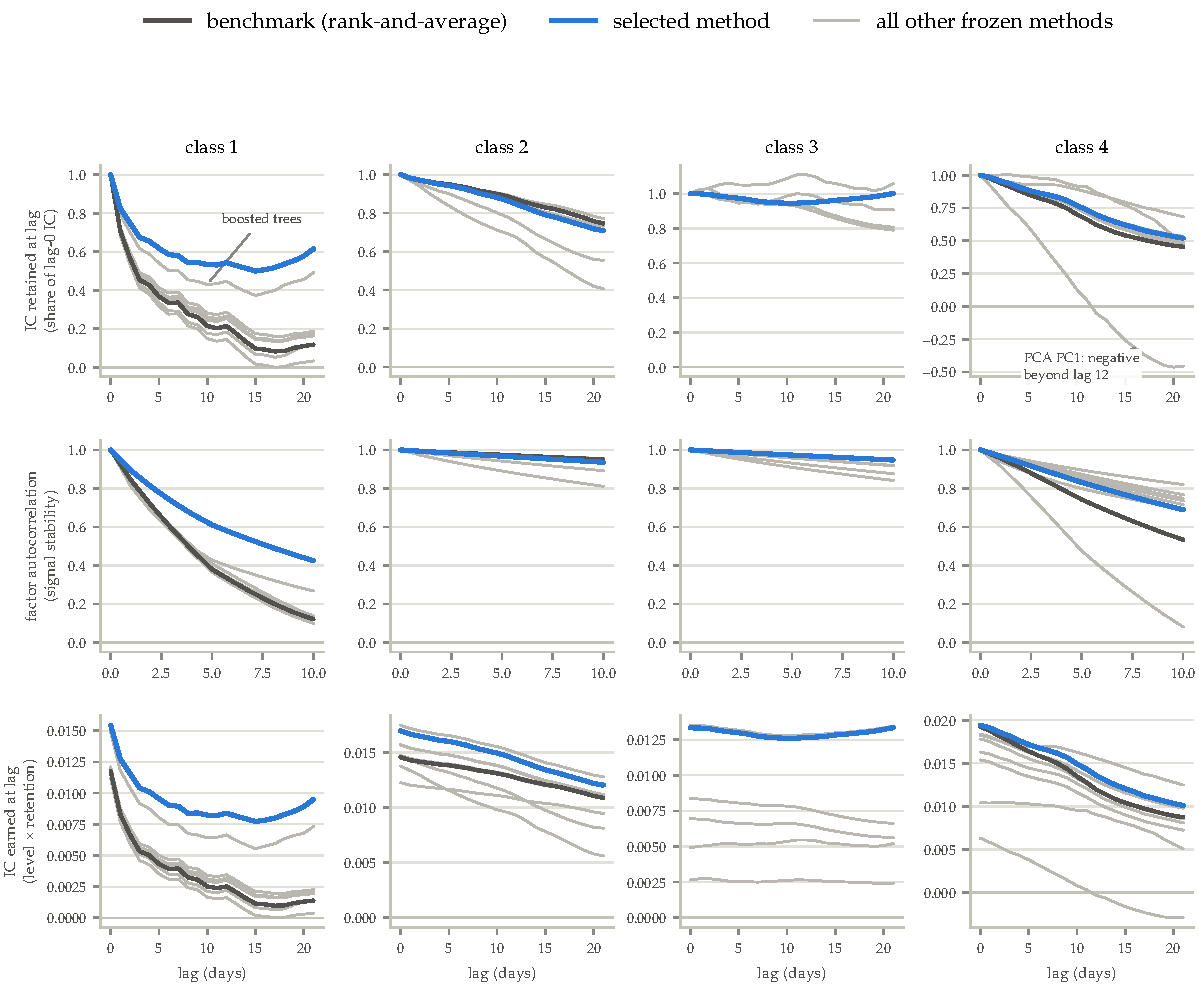
\includegraphics[width=\textwidth]{fig_signallife.pdf}
\caption{The full signal-life record on the blind hold-out, for every frozen method on
every class. Top row: IC retained at each holding lag, as a share of the lag-0 IC.
Middle row: the composite's own autocorrelation at each lag, a measure of how fast the
signal itself changes. Bottom row: IC earned at each lag, the product of level and
retention. Gray is the benchmark, blue the selected method for that class, and thin
light-gray lines all other frozen methods. The class sets the clock: only class~1's
shapes slow it down, and only class~4's PCA breaks it, going negative beyond lag 12.}
\label{fig:signallife}
\end{figure}

\end{document}
